\section*{Preface}
In this chapter, performance of AIBs using two-dimensional molybdenum dichalcogenides as cathodes is discussed. Since molybdenum dichalcogenides have a layered structure, intercalation of chloroaluminates is possible. Bulk (\ce{MoS2}, \ce{MoSe2} and MoSSe) and nanostructured molybdenum dichalcogenides (\ce{MoS2} and \ce{MoSe2}) were tested as cathodes for non- aqueous AIBs and an attempt was made to establish their mechanism. \footnote{Results obtained from this chapter have been published in a pre-print. \textbf{Shalini Divya},James H.Johnston,and Thomas Nann.“Molybdenum Dichalcogenide Cathodes for Aluminium-Ion Batteries”. In: ArXiv191210607 Cond- MatPhysicsphysics (Dec. 2019)}

\pagebreak
\chapter{Molybdenum dichalcogenides as cathodes for rechargeable AIBs} % Main chapter title

\label{chap4} % For referencing the chapter elsewhere, use \ref{Chapter1} 

\section{Theory and background}
Transition metal dichalcogenides (TMDs) have a strong in-plane covalent bonding and weaker van der Waals (vdW) bonds exist between any two layers (similar to graphene layers in graphite). Molybdenum dichalcogenides not only provide redox variability but also a high theoretical capacity (600-1200 mAh g$^{-1}$). The intercalation voltage observed with \ce{MX2}, where M = Mo, W, Ti, etc. and X = S and Se, is high \cite{cong_intrinsic_2015}. The charge storage in TMDs is based on both \enquote{intercalation} and \enquote{conversion-type} mechanisms. To recap, intercalation is where ions insert into the layers of a material during charge and discharge. A conversion-type mechanism is where the material converts itself into an entirely new species every time the cell is, say charged, The new material is converted back to the original material during, say discharge (a reversible process). 
Molybdenum dichalcogenides (\ce{MoX2} where X=S, Se or Te) display similar properties as graphite. They have a layered structure, which allows intercalation of ions. Amongst various transition metal dichalcogenides, \ce{MoS2} has been extensively studied as a cathode for rechargeable batteries \cite{li_mos2_2004, zhu_fast_2015}. Fan \textit{et al.} reported that transition metal dichalcogenide tend to transition from a 2H phase into a more conducting 1T phase when used in a battery \cite{fan_hybrid_2017}. A hybrid \ce{Mg^{2+}}/\ce{Li+} cell was tested using bulk \ce{MoS2} (b-\ce{MoS2}) as a cathode material. The authors proved (using XPS) that the 2H phase-\ce{MoS2} was converted to 1T phase during initial ion intercalation. During cyclic voltammetry (CV) scans, the first cathodic peak, with a phase transition. This seems to be a common phenomenon for molybdenum dichalcogenides, since Li \textit{et al.} observed similar transitions in sodium ion batteries \cite{li_enhancing_2015}. The transition mostly takes place during the first cycle . Since the phase change takes place during the initial stages, it can be detected in the first few scans of a cyclic voltammogram. Molybdenum dichalcogenides have been used as cathodes for non-aqueous AIBs. In 2015, Geng \textit{et al.} found that \ce{Al^3+} ions fully intercalated into chevrel phase \ce{Mo6S8} and the cations occupied two different sites in the crystal lattice \cite{geng_reversible_2015}. The first site was a cubic center of a hexahedron with eight \ce{Mo6S8} units as the vertices, while the second site was face- centered. The cell used a cathode made of \ce{Mo6S8}, an Al anode and an electrolyte consisting of \ce{AlCl3} and butyl-methylimidazolium chloride (\ce{AlCl3}/BMIMCl) with a molar ratio of 1.5:1. The group demonstrated reversible deposition- dissolution of aluminium within the cut-off range of 0.1 and 1.2 V to maintain the stability of the electrolyte and prevent side reactions such as electrolyte degradation. The cell followed a 'rocking chair' mechanism since charge carrying species shuttled back and forth between the electrodes during charge and discharge cycles. The cell displayed an Al intercalation capacity in the first discharge at 148 mAh g$^{-1}$, which quickly stabilised after the first cycle and maintained a capacity of 70 mAh g$^{-1}$ after 50 cycles at an elevated temperature of 50$^{\circ}$C. They reported the physical degradation of \ce{Mo6S8} particles during cycling, which was attributed to the slow capacity fading. They revealed that gradual Al trapping in the \ce{Mo6S8} particles were also responsible for >100\% Coulombic efficiency (CE). The electrochemical reactions displayed by the Al/\ce{Mo6S8} cell at the anode (Eq. \ref{eqan}) and cathode (Eq. \ref{eqcat}) during discharge is reported below \cite{geng_reversible_2015}. \\
\textit{At the anode:} 
\begin{equation} \label{eqan}
\ce{Al + 7AlCl4^- -> 4Al2Cl7^- + 3e^-}
\end{equation}
\textit{At the cathode:}
\begin{equation}\label{eqcat}
\ce{8AlCl7^- + 6e^- + Mo6S8 -> Al2Mo6S8 + 14AlCl4^-}
\end{equation}
A new complex was \ce{Al2Mo6S8} was formed during discharge when \ce{Mo6S8} reacted with \ce{Al2Cl7-} ions from the electrolyte. Three years later, Li and his group prepared \ce{MoS2} microspheres via a simple hydrothermal method \cite{li_rechargeable_2018}. They proposed a similar mechanism where \ce{Al^3+} ions inserted into the \ce{MoS2} cathode accompanied by a phase transformation at the electrode interface during discharge. They confirmed the phase- transition by using \textit{ex-situ} XPS and XRD techniques. The \ce{MoS2} microspheres exhibited low CE, which was attributed to the \ce{MoS2} phase transition and formation of an solid electrolyte interface (SEI) film. The formation of an SEI layer prevents the cathode from further participating in the electron transfer processes. Also, a low CE indicates presence of side reactions and/or cathode degradation. At a current rate of 40 mA g$^{-1}$, the cell maintained a specific capacity of 77 mAh g$^{-1}$ during discharge for 100 cycles with CE of $\sim$90\%. They also pointed out at the large difference between the charge and discharge curves. The phenomena was a result of \lq electrochemical polarization\rq caused by large charge density of \ce{Al^3+} under electrostatic effects during the cycles. The electrochemical reaction for this battery system (during discharge) was described by the following equations. \\
\textit{At the cathode:}
\begin{equation}
    \ce{MoS2} + \ce{Al^{3+}} + 3\ce{e- -> Al_xMoS2}
\end{equation}
\textit{At the anode:}
\begin{equation}
    \ce{Al} + 7\ce{AlCl4- ->} 4\ce{Al2Cl7-} + 3\ce{e-}
\end{equation}

In general, aluminium batteries that used molybdenum disulfide as cathodes showed low energy density and had reversibility issues during the redox processes. 

This chapter documents a range of bulk and nanostructured 2D molybdenum dichalcogenides including molybdenum disulfide (\ce{MoS2}), molybdenum diselenide (\ce{MoSe2}) and molybdenum sulfide selenide (\ce{MoSSe}), as cathodes for non-aqueous AIBs at room temperature. The preliminary density functional theory (DFT) calculations performed by Professor Thomas Nann in The University of Newcastle indicated a significant decrease in the inter-layer spacing of molybdenum dichalcogenides when \ce{Al^3+} cations were assumed to intercalate (owing to the very high charge density of \ce{Al^3+}). Therefore, intercalation of structurally distorted \ce{AlCl4-} anions into the \ce{MoX2} cathode layers is proposed. Surprisingly, it was found that \ce{MoSe2}-based cathodes performed better than all of the other molybdenum dichalcogenides.

\section{Experimental methods}
Refer to Sections \ref{slurry}, \ref{catprep}, \ref{vac} and \ref{cellass} for cathode preparation and cell assembly methods. 

\section{Results and Discussion}
Figure \ref{Figures/chap4fig:S1} shows the crystal structure of \ce{MoX2} where X is sulfur (S) and/or selenium (Se). The material has two vacant sites for intercalation --- M1 and M2. M1 denotes the spaces in between the X-Mo-X atoms, whereas M2 represents the space created between the \ce{MoX2} layers as shown in Figure \ref{Figures/chap4fig:1} a. The inter-layer distance in \ce{MoX2} is 6.3 \AA\ with a gallery height of 3 \AA. The layers are held together by van der Waals (vdW) forces. M2 presents an open network and provides various interstitial sites for intercalation. Since \ce{AlCl4-} ions are 5.28 \AA\ in diameter, as reported by Takahashi {\it et al.} \cite{takahashi_niv2o5nh2o_2005}, they must undergo some distortion during intercalation to fit into these layers. The preliminary DFT results showed that \ce{Al^{3+}} would \lq contract\rq\ the \ce{MoX2} layers when trying to intercalate, making \ce{AlCl4-} anion intercalation more likely. Also, the triply charged \ce{Al^{3+}} cation has to overcome strong electrostatic forces from the \ce{S^{2-}} or \ce{Se^{2-}} anion network in order to enter, making the intercalation process slow and most likely not reversible. Therefore, intercalation of \ce{AlCl4-} anions from the electrolyte into M2 sites of \ce{MoX2} during charge is proposed. Galvanostatic cycles, cyclic voltammetry (CV), X-Ray diffraction (XRD), Raman spectra and X-Ray Photoelectron Spectroscopy (XPS) results discussed later, strongly support reversible electron transfer processes occurring especially in \ce{MoSe2}.

\begin{figure}
  \centering
  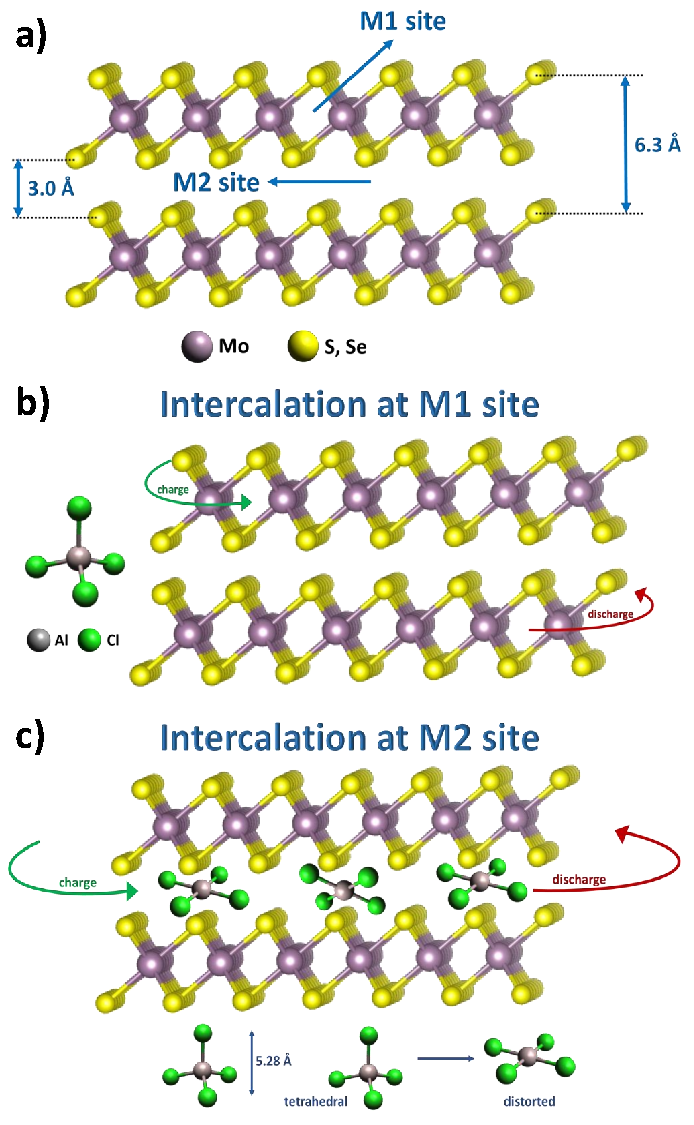
\includegraphics[width=\textwidth]{Figures/chap4fig/s1}
  \caption{Schematic representation of a) a \ce{MoX2} crystal structure with possible intercalation sites at M1 and M2 b) intercalation at M1 site and c) intercalation at M2 site.}
  \label{Figures/chap4fig:s1}
\end{figure}

\begin{figure}[htb!]
\centering
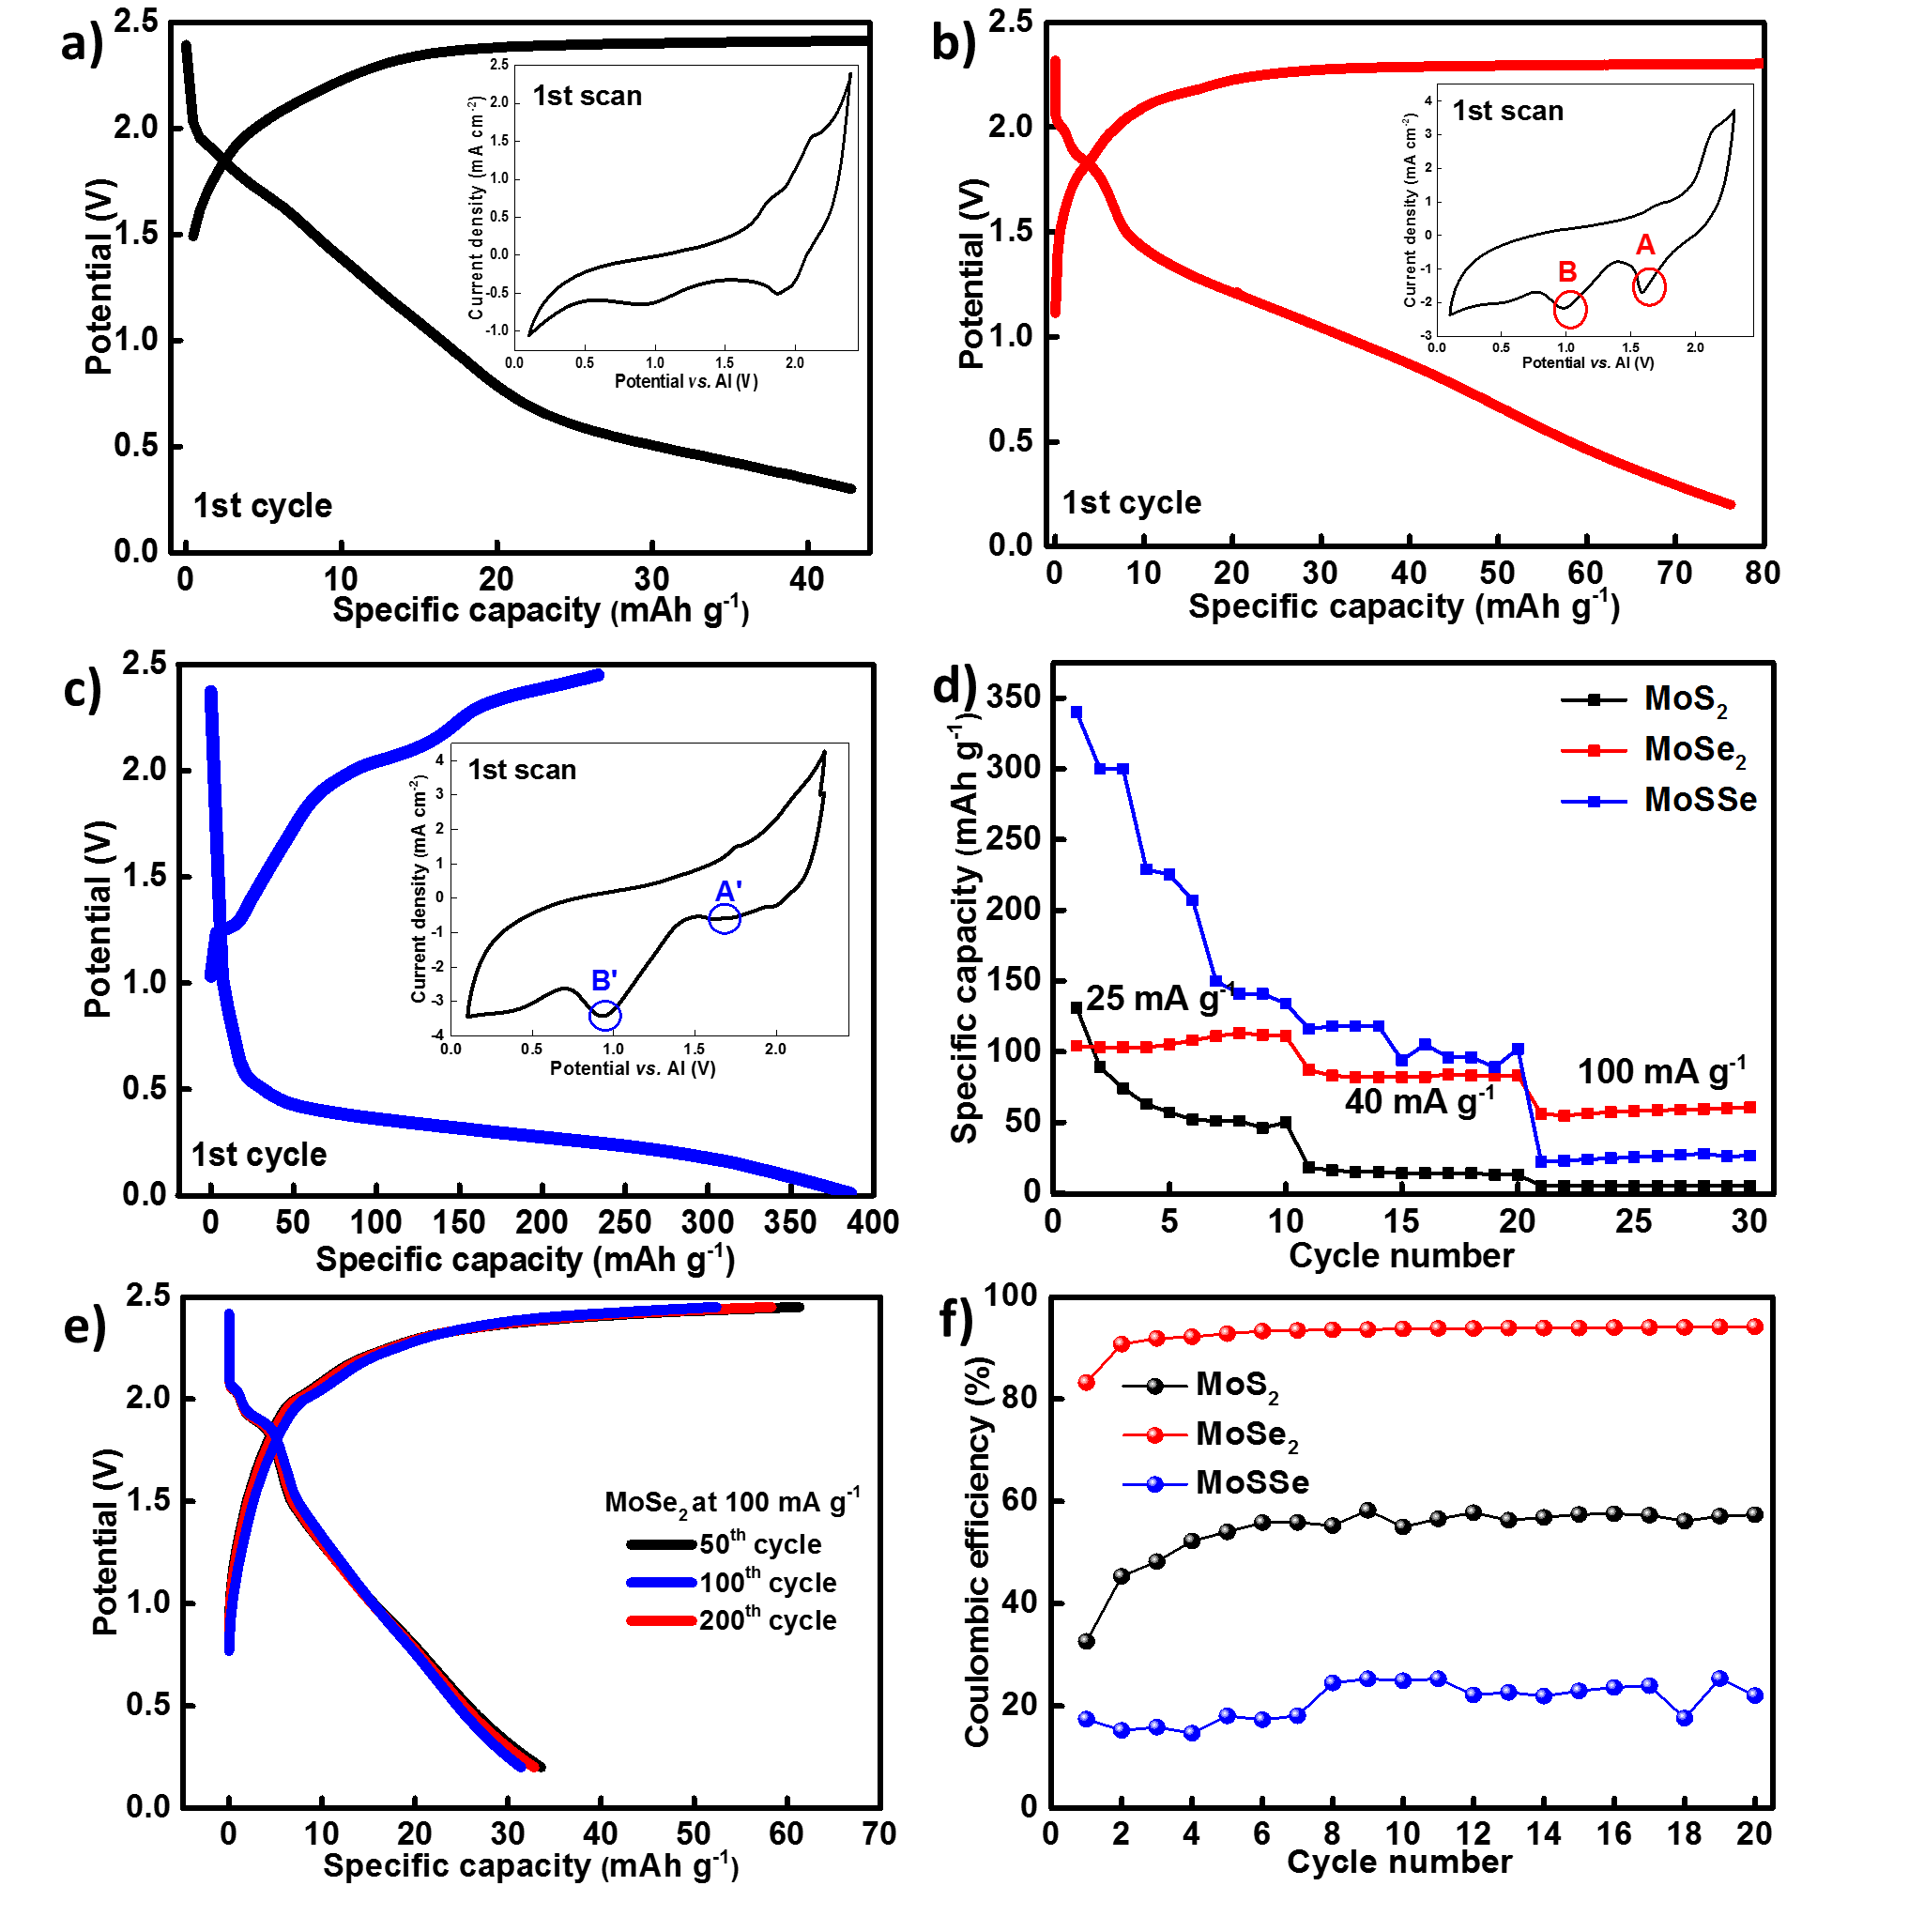
\includegraphics[width=\textwidth]{Figures/chap4fig/MoX2CDCCV}
\caption{First charge/discharge curve at 40 mA g$^{-1}$ for a) \ce{MoS2}, b) \ce{MoSe2} and c) MoSSe. d) Specific capacities of \ce{MoS2}, \ce{MoSe2} and MoSSe at current rates of 25, 40 and 100 mA g$^{-1}$. \textit{Figure \ref{Figures/chap4fig:MoX2CDCCV} a inset}- first CV scan of \ce{MoS2}, \textit{Figure \ref{Figures/chap4fig:MoX2CDCCV} b inset}- first CV scan of \ce{MoSe2} and \textit{Figure \ref{Figures/chap4fig:MoX2CDCCV}c inset}- first CV scan of MoSSe at a scan rate of 10 mV s$^{-1}$ in an aluminium-ion battery against Al reference electrode. e) Charge/ discharge curves of Al/\ce{MoSe2} cell at a high current rate of 100 mA g$^{-1}$ for 200 cycles. f) CEs of \ce{MoS2} (in black), \ce{MoSe2} (in red) and MoSSe (in blue).}
\label{Figures/chap4fig:MoX2CDCCV}
\end{figure} 

Figure \ref{Figures/chap4fig:MoX2CDCCV} a--c shows the charge/discharge cycles (CDCs) for \ce{MoS2}, \ce{MoSe2} and MoSSe at a current rate of 40 mA g$^{-1}$. The discharge capacity of Al/\ce{MoS2} in its first cycle was found at $\sim$45 mAh g$^{-1}$, Figure \ref{Figures/chap4fig:MoX2CDCCV} a). Comparing this with its first CV scan (Figure \ref{Figures/chap4fig:MoX2CDCCV} g, a good correlation between the discharge voltage plateau and reduction peaks, and other redox features was found. This suggested that an electron transfer process (intercalation and/or conversion) was taking place at that voltage. Lin \textit{et al.} proved that a voltage plateau was formed at 2.0 V when the \ce{AlCl4-} ions intercalated into the graphite layers. Corresponding to that voltage, a redox peak was observed in the cell's CV scan, which confirmed the occurrence of a redox reaction at 2.0 V. With discharge plateaus at 1.9 V and 1.7 V, the first CV scan for \ce{MoSe2} displayed two reduction peaks at 1.65 V (point A) and 1.0 V (point B), Figures \ref{Figures/chap4fig:MoX2CDCCV} b and \ref{Figures/chap4fig:MoX2CDCCV} h. The peak at 1.0 V suggested an irreversible reaction since this peak was absent in the following scans. \\
Based on Li \textit{et al.}'s interpretation of the cyclic voltammogram, this peak was attributed to an irreversible phase transition \cite{li_enhancing_2015}. During this transition, the semi-conducting 2H phase of \ce{MoSe2} converted into a more metallic 1T phase. \\
Following Fan \textit{et al.}'s reports, it was assumed that the 2H\ce{->}1T phase transition might have increased the interlayer spacing of \ce{MoSe2} by reducing the vdW forces that exist between the two layers \cite{fan_hybrid_2017}. \\
Al/MoSSe cells showed three distinct plateaus during charging at 1.2 V, 2.0 V and 2.3 V in its first cycle, with a discharge plateau at 0.5 V shown in Figure \ref{Figures/chap4fig:MoX2CDCCV} c. Capacities of all molybdenum dichalcogenides were recorded at different current rates of 25, 40 and 100 mA g$^{-1}$, and displayed in Figure \ref{Figures/chap4fig:MoX2CDCCV} d. For \ce{MoSe2}, a highly reversible electrochemical reaction was observed as the capacity remained at 30-32 mAh g$^{-1}$ after 200 cycles at a high current rate of 100 mA g$^{-1}$ (Figure \ref{Figures/chap4fig:MoX2CDCCV} e). The presence of multiple charging plateaus in MoSSe might correspond to various oxidation processes occurring when \ce{AlCl4-} interacts individually with S and Se atoms. \\
The first CV scan in Figure \ref{Figures/chap4fig:MoX2CDCCV} c- inset showed an irreversible reduction potential at $\sim$1.0 V, point B', like \ce{MoSe2}, implying a similar phase transition. It seems MoSSe undergoes a lattice distortion and the material loses its \enquote{long-range order} after converting to its 1T phase. This might be the reason why the cells failed to deliver a stable capacity. In addition, a significant difference was observed between the charging and discharging curves of all the molybdenum cathodes, similar to what was previously reported by Li \textit{et al.} in 2018. This suggested the presence of electrochemical polarization at the electrode interface. %Advanced techniques are needed to study those differences and reduce it. 
CVs of a blank cell with an uncoated Mo foil (Figure \ref{Figures/appendix:blankmol}) showed that the current collector did not contribute to the cell's capacity. \\
Both \ce{MoS2} and \ce{MoSe2} have similar interlayer distance (6.3 \AA) and a gallery height of 3.0 \AA. However, \ce{MoSe2} showed a higher capacity and a more stable cycle life. To account for this behaviour, the cyclic voltammograms of all electrodes was compared at a scan rate of 10 mV s$^{-1}$ in Figure \ref{Figures/chap4fig:fig2}. Different charge-storage mechanisms lead to distinct features in the CVs. Ideal capacitors result in a rectangular CV shape. Due to the absence of Faradaic processes (oxidation and/or reduction at the electrode), the charging/discharging currents become directly proportional to the scan speed. Batteries show oxidation and reduction peaks in their voltammograms because the charge storage takes place via certain redox processes \cite{jiao_aluminum-ion_2016}. It was observed that the CVs of \ce{MoSe2} and MoSSe in Figure \ref{Figures/chap4fig:fig2} b and \ref{Figures/chap4fig:fig2} c covered a broader area suggesting an additional capacitor-like charge storage mechanism. This additional non-Faradaic process taking place at their surfaces might have attributed to the higher capacities for \ce{MoSe2} and  MoSSe. Also, the peak indicating phase transition from 2H$\rightarrow$1T at $\sim$0.9 -1.0 V was visible only for \ce{MoSe2} and MoSSe. Hence, it can be concluded that the charge storage in \ce{MoS2} is primarily based on reversible oxidation and reduction of Mo from \ce{Mo^{4+}} to \ce{Mo^{5+}} with oxidation peaks visible at 1.8 V (O1) and 2.1 V (O2), and a corresponding reduction peak at 2.0 V (R3), Figure \ref{Figures/chap4fig:fig2} a. Two more reduction peaks were found at 1.6 V (R2) and 0.9 V (R1). However, their peak intensities decreased with every scan. The oxidation and reduction peaks in a cyclic voltammogram should be reproducible if done for a reversible reaction, i.e. no side reactions are taking place depleting the active species.\\
Sometimes, deposition on the electrode hampers the advancement of the electrochemical reactions, which results in redox peaks that do not coincide with each other. It seems something similar happened at R1 and R2. CV scans of Al/\ce{MoSe2} cells in Figure \ref{Figures/chap4fig:fig2} b indicated a reversible electrochemical process. The scans overlapped with each other displaying two oxidation peaks at 1.7 V (O'1) and 2.1 V (O'2) and corresponding reduction peaks at 1.8 V (R'1) and 1.6 V (R'2), which corresponded well with the voltage bends and plateaus observed in the charge/ discharge cycles. In Figure \ref{Figures/chap4fig:fig2} c an oxidation and a reduction peak at 1.7 V (O''1) and 1.8 V (R''1) was observed for Al/MoSSe respectively. R''1's peak intensity increased after every scan, which might suggest sluggish kinetics in the system; perhaps due to strong interaction between the host material and the intercalating anion. The voltammogram became more capacitor-like after a few scans, indicating the absence of reversible redox processes. The phenomena indicates that an initial intercalation process was followed by surface-adsorption of \ce{AlCl4-} anions , resulting in a capacitor-like charge storage. 

\begin{figure}
  \centering
  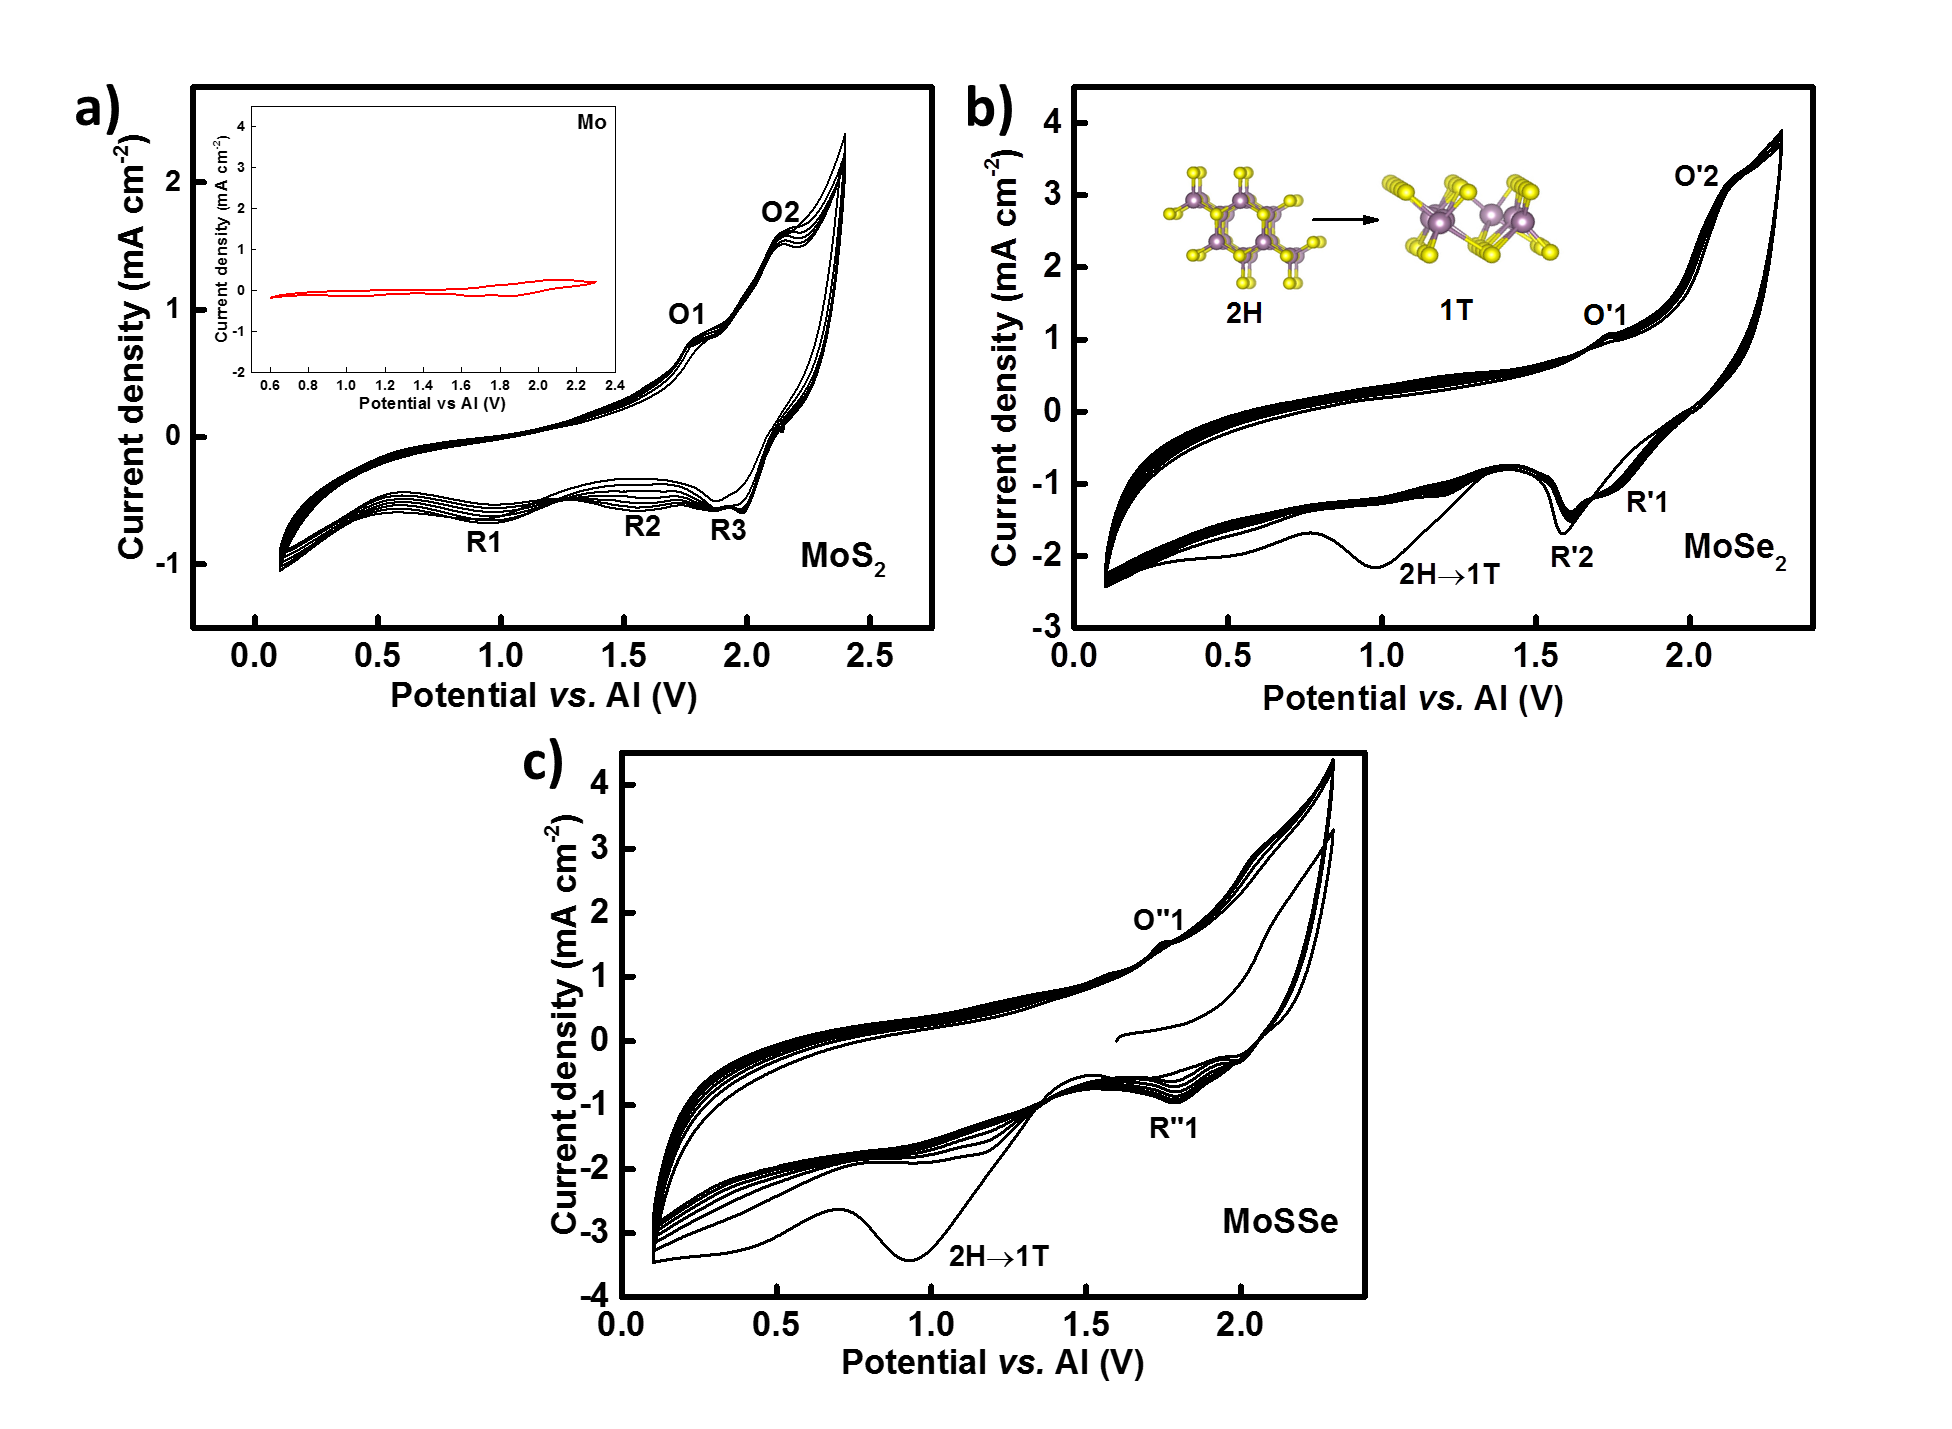
\includegraphics[width=\textwidth]{Figures/chap4fig/fig2}
  \caption{Cyclic voltammograms of a) \ce{MoS2}, b) \ce{MoSe2} and c) MoSSe at a scan rate of 10 mV s$^{-1}$ in a two-electrode aluminium-ion cell against an Al/\ce{Al^{3+}} reference electrode.}
  \label{Figures/chap4fig:fig2}
\end{figure} 

\begin{figure}
  \centering
  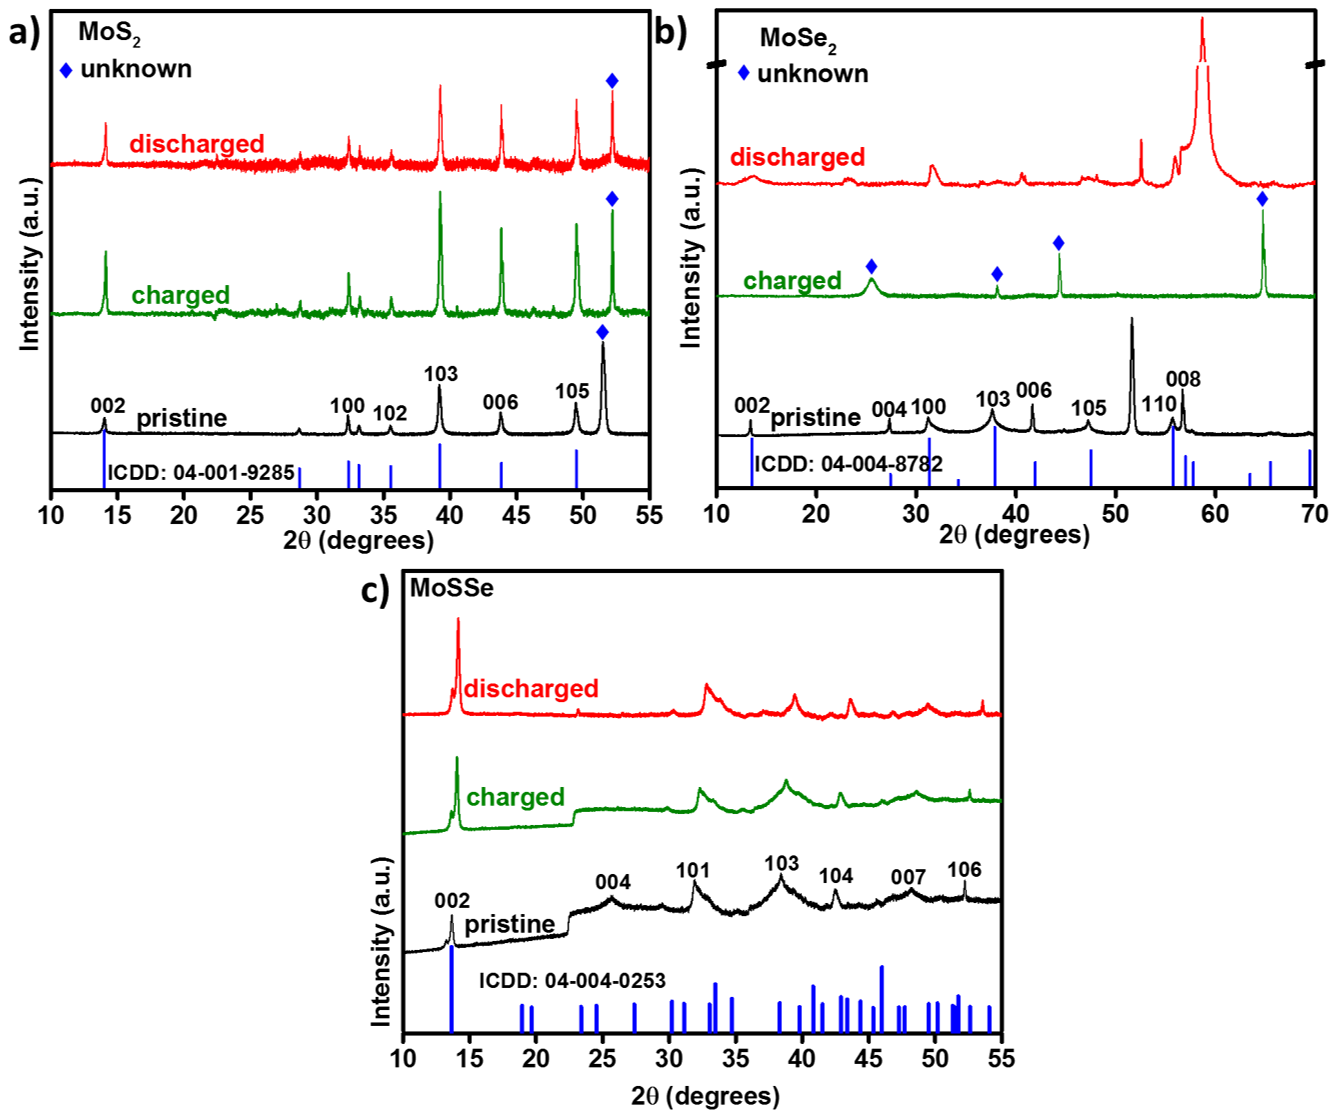
\includegraphics[width=\textwidth]{Figures/chap4fig/fig3}
  \caption{X-ray diffraction patterns of pristine (black), charged (green) and discharged (red) a) \ce{MoS2}, b) \ce{MoSe2} and c) MoSSe electrodes charged to 2.35 V and discharged to 0.2 V vs. Al/\ce{Al^{3+}}, with International Centre for Diffraction Data (ICDD) references in blue.}
  \label{Figures/chap4fig:fig3}
\end{figure}

Figure \ref{Figures/chap4fig:fig3} shows the XRD patterns of \ce{MoS2}, \ce{MoSe2} and MoSSe electrodes. Pristine (in black), charged (in green) and discharged (in red) cathodes were compared after 30 cycles each. \ce{MoS2} cells displayed a very small shift in their d-spacings. The peak at 14.2$^{\circ}$ (6.22 \AA) shifted to 14.02$^{\circ}$ (6.32 \AA), as shown in Figure \ref{Figures/chap4fig:fig3} a. Most of the peaks retained their positions after charge and discharge showing no significant change in the lattice dimensions. A completely different XRD pattern appeared after charging for Al/\ce{MoSe2} cells, as new peaks appeared at 2$\theta$ values, displayed in Figure \ref{Figures/chap4fig:fig3} b. After discharge, the diffraction patterns of the cathodes resembled the pristine cathode patterns. Every time the cells were charged, \ce{MoSe2} seemed to adopt this new crystal lattice. However, the characteristic peaks of \ce{MoSe2} reappeared after discharge. This follows closely the observations made by Rani \textit{et al.} \cite{rani_fluorinated_2013}, where they proved intercalation of ions into the layers of fluorinated natural graphite during charging. This strongly confirmed the hypothesis of a reversible intercalation and/or conversion-type mechanism was taking place in \ce{MoSe2}. It was interesting to note that MoSSe did not have a well-defined crystal structure to begin with, Figure \ref{Figures/chap4fig:fig3} c. The patterns after charge and discharge did not look any different from the untested cathode. This confirmed MoSSe layers did not undergo any significant expansion and the initial high specific capacities ($\sim$250 mAh g$^{-1}$)came from non-Faradaic reactions where \ce{AlCl4-} might have been electrostatically absorbed onto the surface of the electrode. Furthermore, the cells underwent irreversible processes since they became inactive after a few cycles suggesting complete cathode degradation. 
\begin{figure}
  \centering
  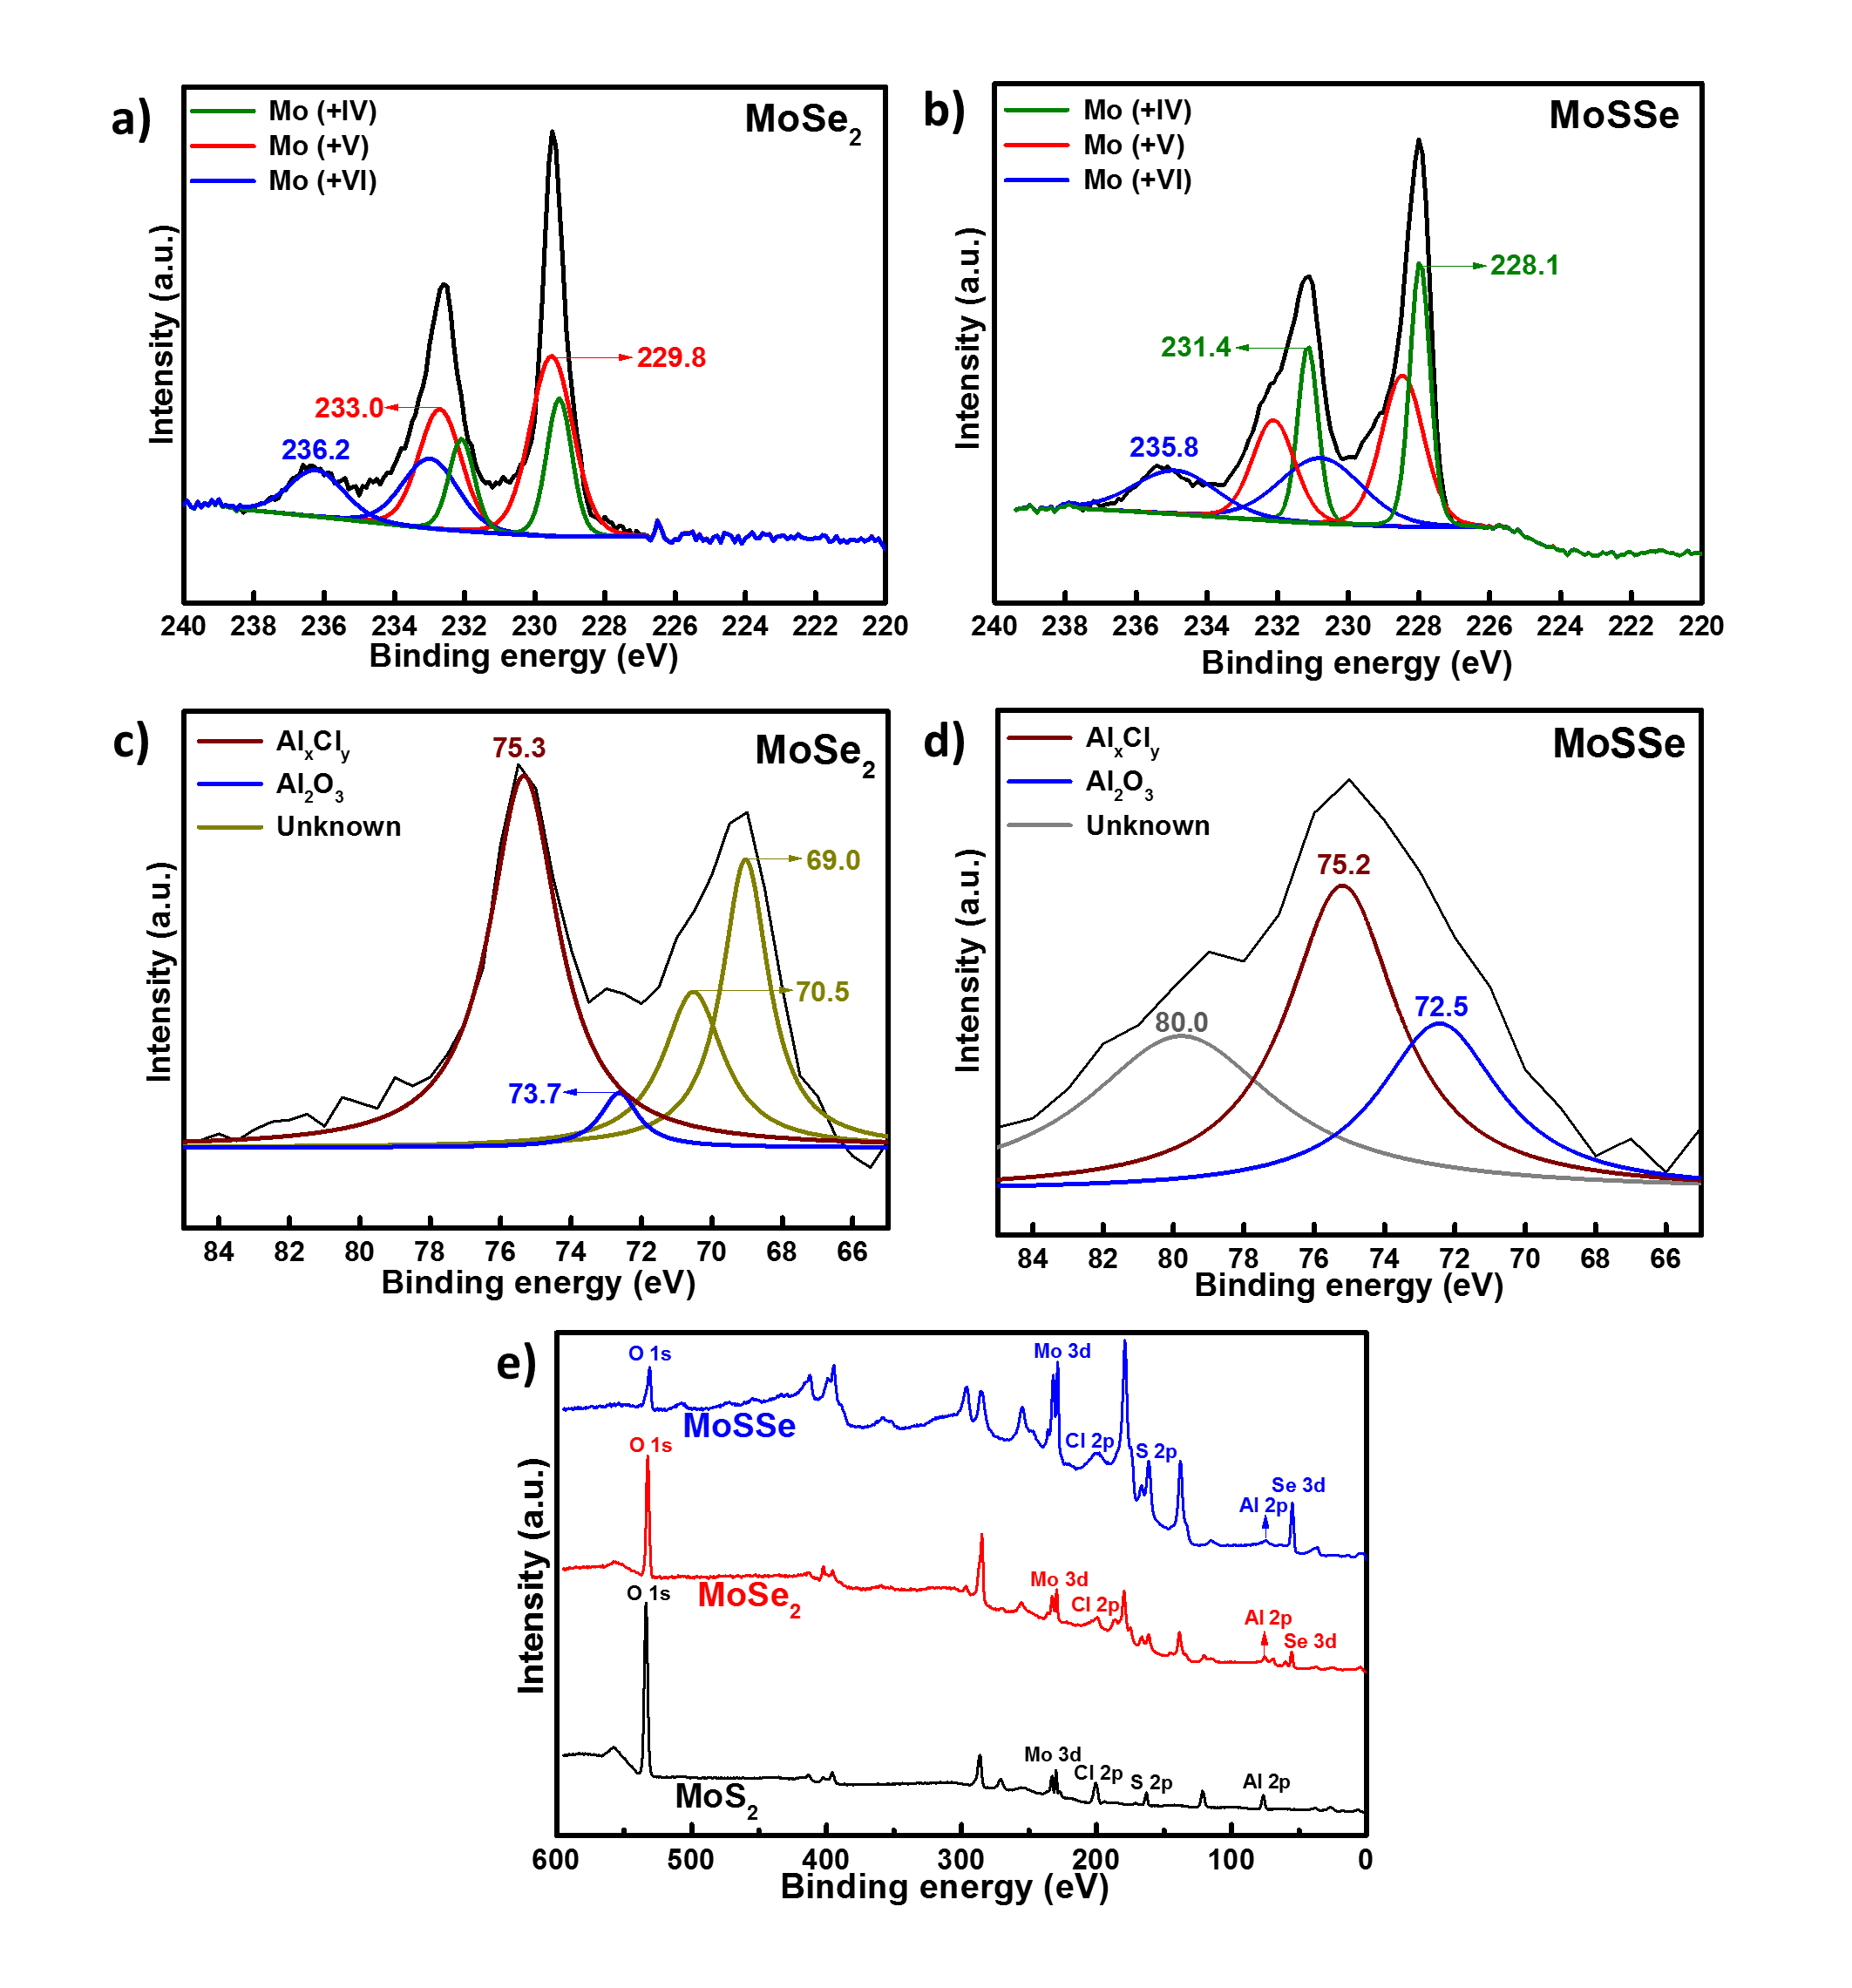
\includegraphics[width=\textwidth]{Figures/chap4fig/MoAlOverallMoSeMoSSe}
  \caption{XPS spectra of Mo 3d orbitals in a charged a) \ce{MoSe2} and b) MoSSe cathode and Al 2p orbitals in a charged c) \ce{MoSe2} and d) MoSSe cathode. e) An overview spectrum of all three charged cathodes.}
  \label{Figures/chap4fig:MoAlOverallMoSeMoSSe}
\end{figure}
To further understand the interactions between \ce{AlCl4-} and \ce{MoSe2}, XPS was used, which is a useful method for distinguishing various oxidation states and helps in identifying different polymorphs (2H and 1T) \cite{fan_hybrid_2017}. The detailed narrow spectrum scans in Figure \ref{Figures/chap4fig:MoAlOverallMoSeMoSSe} show the binding energies of Mo (3d$_{5/2}$ and 3d$_{3/2}$ in Figure \ref{Figures/chap4fig:MoAlOverallMoSeMoSSe} a and b, and Al 2p peaks for charged \ce{MoSe2} in Figure \ref{Figures/chap4fig:MoAlOverallMoSeMoSSe} c and MoSSe electrodes in Figure \ref{Figures/chap4fig:MoAlOverallMoSeMoSSe} d. In pristine \ce{MoSe2}, two peaks appeared at 229.1 eV and 232.2 eV corresponding to 3d$_{5/2}$ and 3d$_{3/2}$ (Figure\ \ref{Figures/chap4fig:MoSeSeAlClPrtChg} a)). Selenium displayed a doublet at 55.4 eV and 54.6 eV corresponding to Se 3d$_{3/2}$ and 3d$_{5/2}$ respectively (Figure \ref{Figures/chap4fig:MoSeSeAlClPrtChg} c). Peak splitting in an XPS spectrum typically indicates a phase change or a change in the oxidation state of the said element. After charging, the peak for Mo 3d split into three doublets indicating the presence of multiple oxidation states or phases of Mo (Figure \ref{Figures/chap4fig:MoAlOverallMoSeMoSSe} a). Se 3d deconvoluted into four peaks after charge, Figure \ref{Figures/chap4fig:MoSeSeAlClPrtChg} e, confirming presence of more than one phase after charge. This was similar to observations made by Fan and his group, when they used \ce{MoS2}/graphene cathode in a hybrid \ce{Mg^2+}/\ce{Li+} cell \cite{fan_hybrid_2017}. Pristine electrodes of MoSSe contained Mo in more than one oxidation state, and provided evidence for the presence of both 2H and 1T polymorphs, Figure\ \ref{Figures/chap4fig:MoSeSeAlClPrtChg} b. After charging, the width of peaks at 231.7 and 228.6 eV (in green, corresponding to Mo 3d$_{5/2}$ and Mo 3d$_{3/2}$ respectively) increased as displayed in Figure\ \ref{Figures/chap4fig:MoAlOverallMoSeMoSSe} b. After comparing Figure\ \ref{Figures/chap4fig:MoSeSeAlClPrtChg} d and f, it was noticed that the Se 3d spectrum deconvoluted into four peaks after charging in MoSSe cells. An increase in the peak width was observed for both Mo and Se binding energies. A new peak at $\sim$236 eV in Mo 3d spectra (in blue) for \ce{MoS2}, \ce{MoSe2} and MoSSe electrodes was assigned to Mo$^{6+}$ species generally present in molybdenum oxide, \ce{MoO3}. 
\begin{figure}
  \centering
  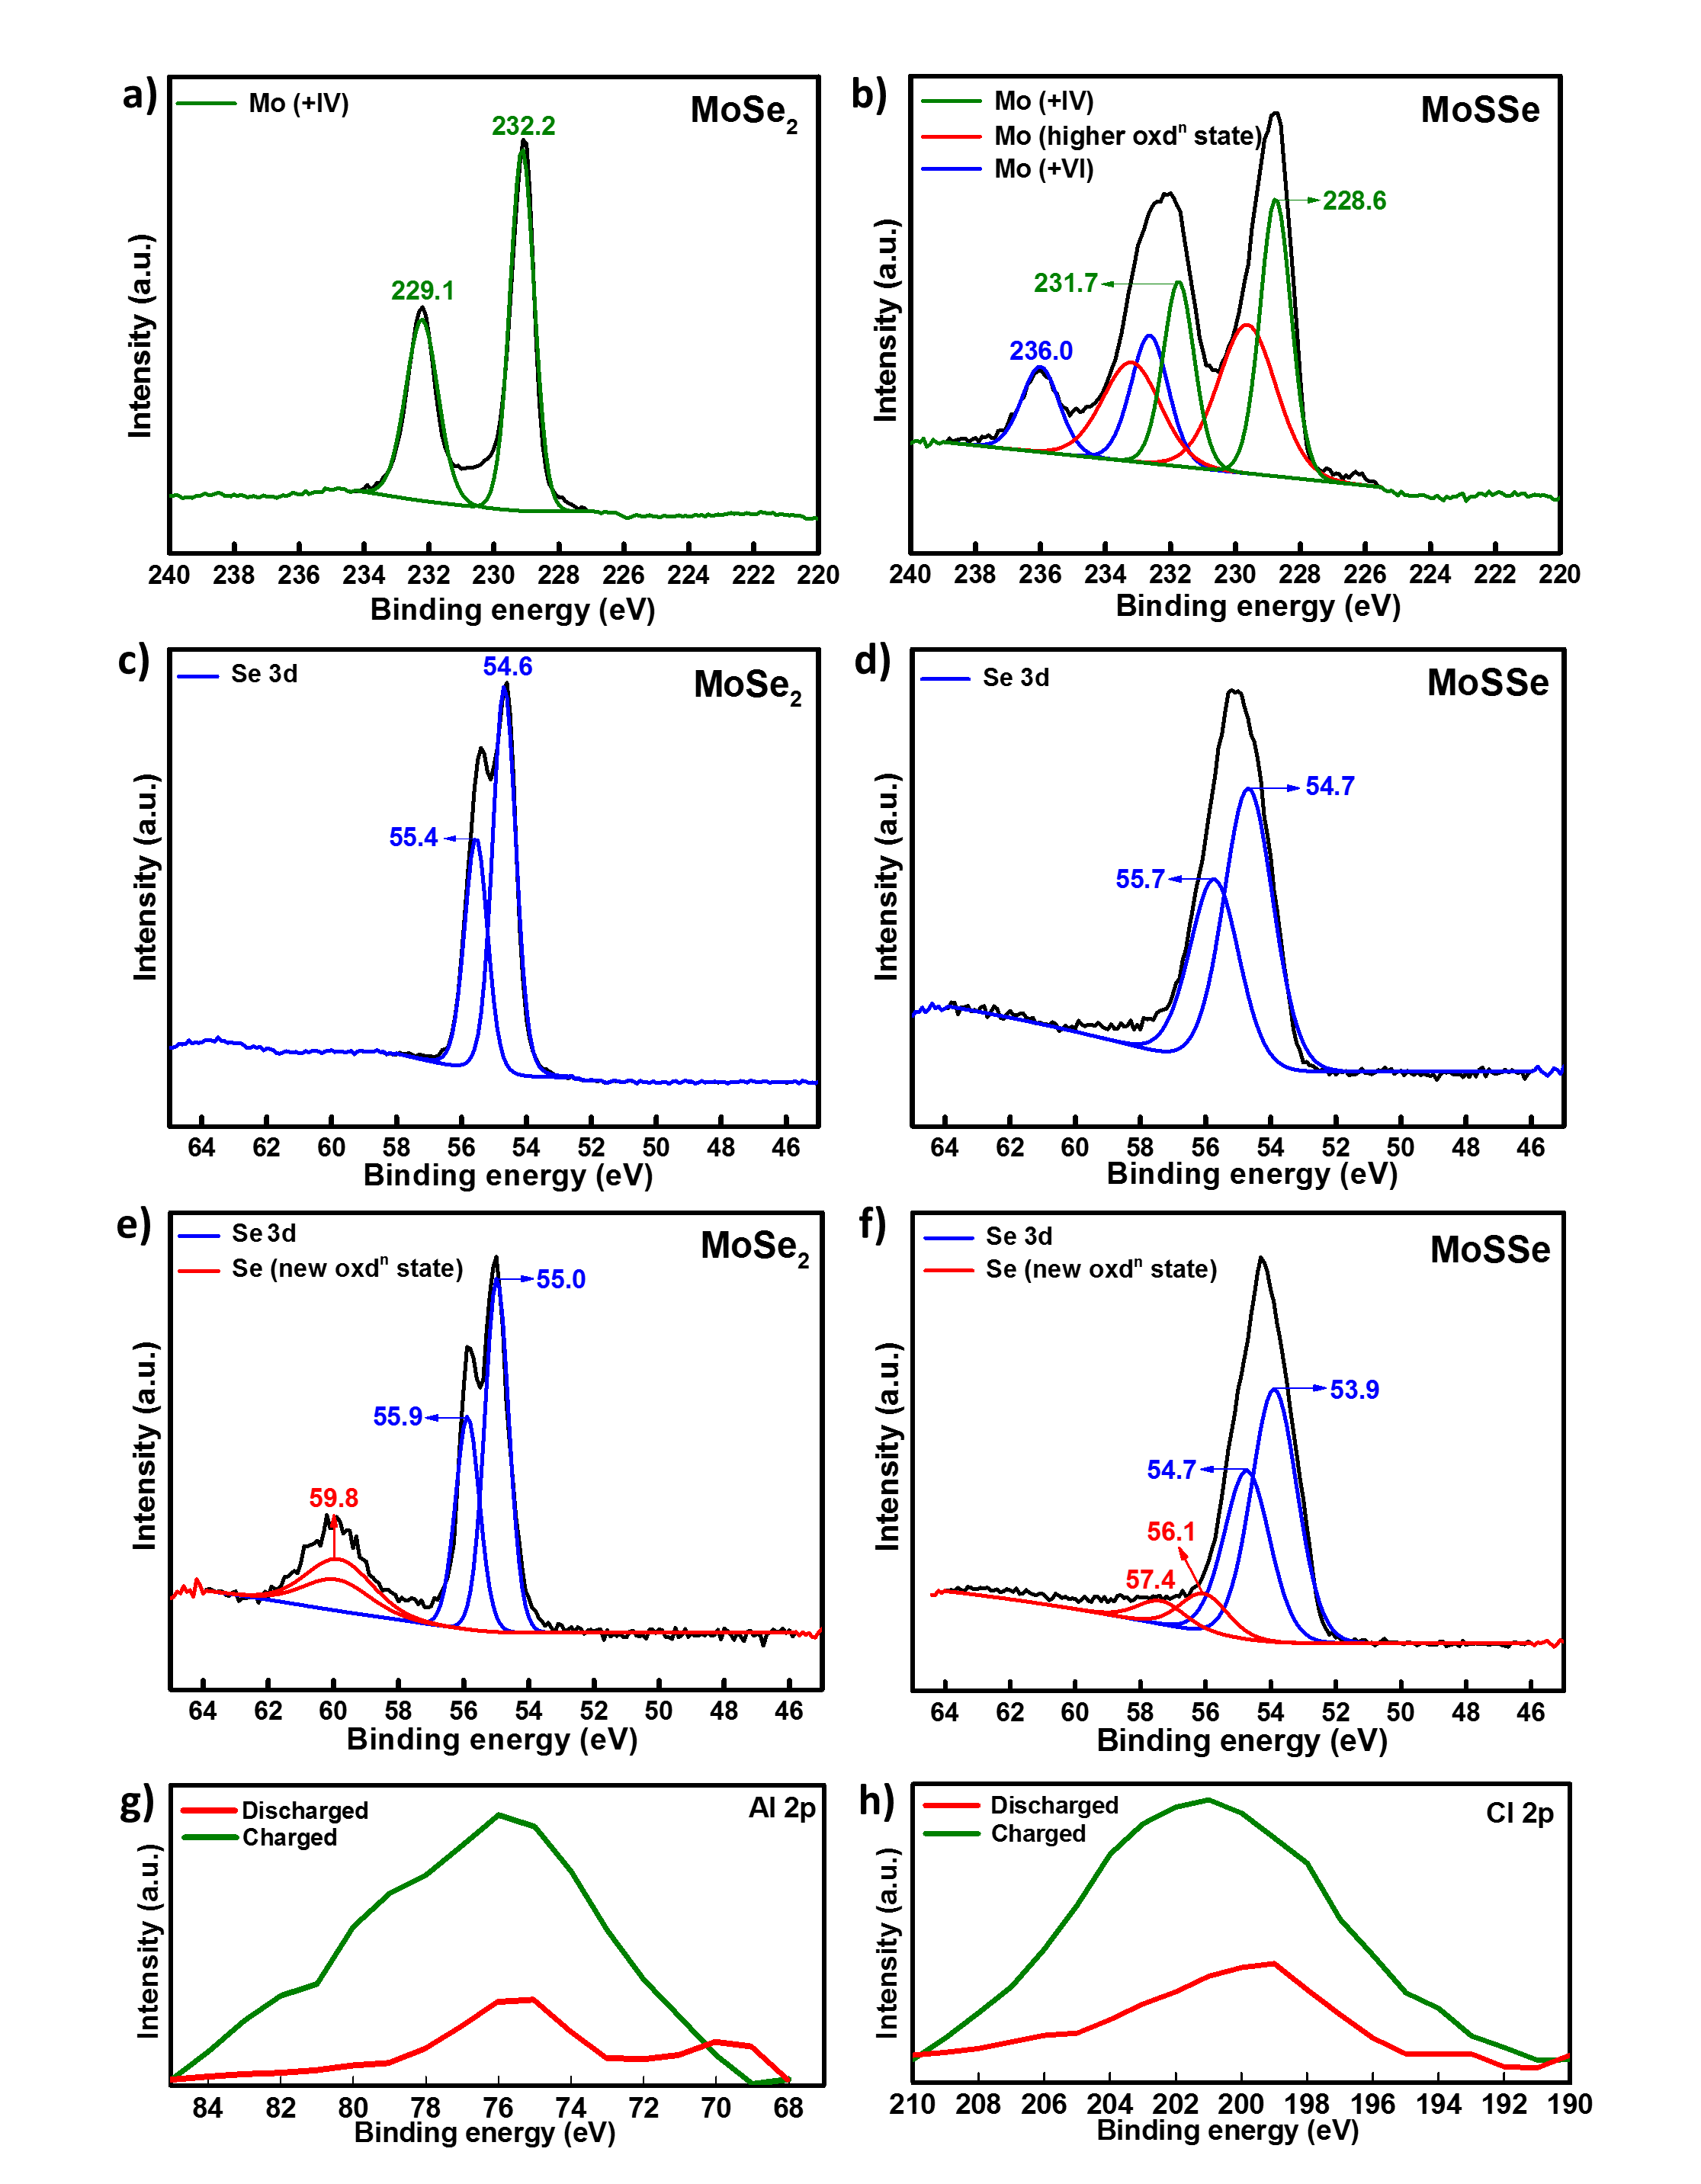
\includegraphics[width=0.9\textwidth]{Figures/chap4fig/MoSeSeAlClPrtChg}
  \caption{XPS spectra of Mo 3d for pristine a) \ce{MoSe2} and b) MoSSe electrodes. The spectra of \ce{MoSe2} are composed of two peaks at 232.2 eV and 229.1 eV corresponding to \ce{Mo^{4+}}. MoSSe spectra consist of three doublet bands, which were assigned to \ce{Mo^{4+}}, one with higher oxidation state and another band corresponding to \ce{Mo^{6+}} at 236 eV. c) Pristine and e) charged Se 3d from \ce{MoSe2}. \ce{MoSe2} observed peaks corresponding to 3d$_{3/2}$ and 3d$_{5/2}$ at 55.6 eV and 54.6 eV respectively. Binding energies of Se 3d from d) pristine and f) charged MoSSe cathodes.}
  \label{Figures/chap4fig:MoSeSeAlClPrtChg}
\end{figure}
The peak shifts detected in Mo 3d spectra for charged \ce{MoS2} and \ce{MoSe2} cathodes were insignificant in MoSSe since no new peaks appeared in the Mo 3d spectra for MoSSe. This further confirms the absence of redox reactions and that the capacity was mainly derived from a surface-based charge storage. As expected, a general trend was observed for all the three cathodes, where the charged electrodes showed higher concentration of aluminium and chlorine than discharged electrodes shown in Figure \ref{Figures/chap4fig:MoSeSeAlClPrtChg} g and h. The XPS spectra support the observation that \ce{MoSe2} underwent a phase transformation that made it a better performing cathode than \ce{MoS2}. Further analysis is needed to fully understand the mechanism of MoSSe.

Charged \ce{MoSe2} electrodes displayed binding energies of Al 2p at 75.3 eV (red) and 73.7 eV (in blue) corresponding to chloroaluminates (\ce{Al_xCl_y}) and aluminium oxide (\ce{Al2O3}) respectively in Figure \ref{Figures/chap4fig:MoAlOverallMoSeMoSSe} c. New peaks were observed at much lower binding energies --- 69 and 70.5 eV (green) suggesting the presence of a new complex with an increased electron density around aluminium. The new complex might be the product of the conversion reaction that takes place. An overall spectra of charged \ce{MoS2}, \ce{MoSe2} and MoSSe cathodes is shown in Figure \ref{Figures/chap4fig:MoAlOverallMoSeMoSSe} e indicating the presence of Al and Cl (from chloroaluminates).
\begin{figure}
  \centering
  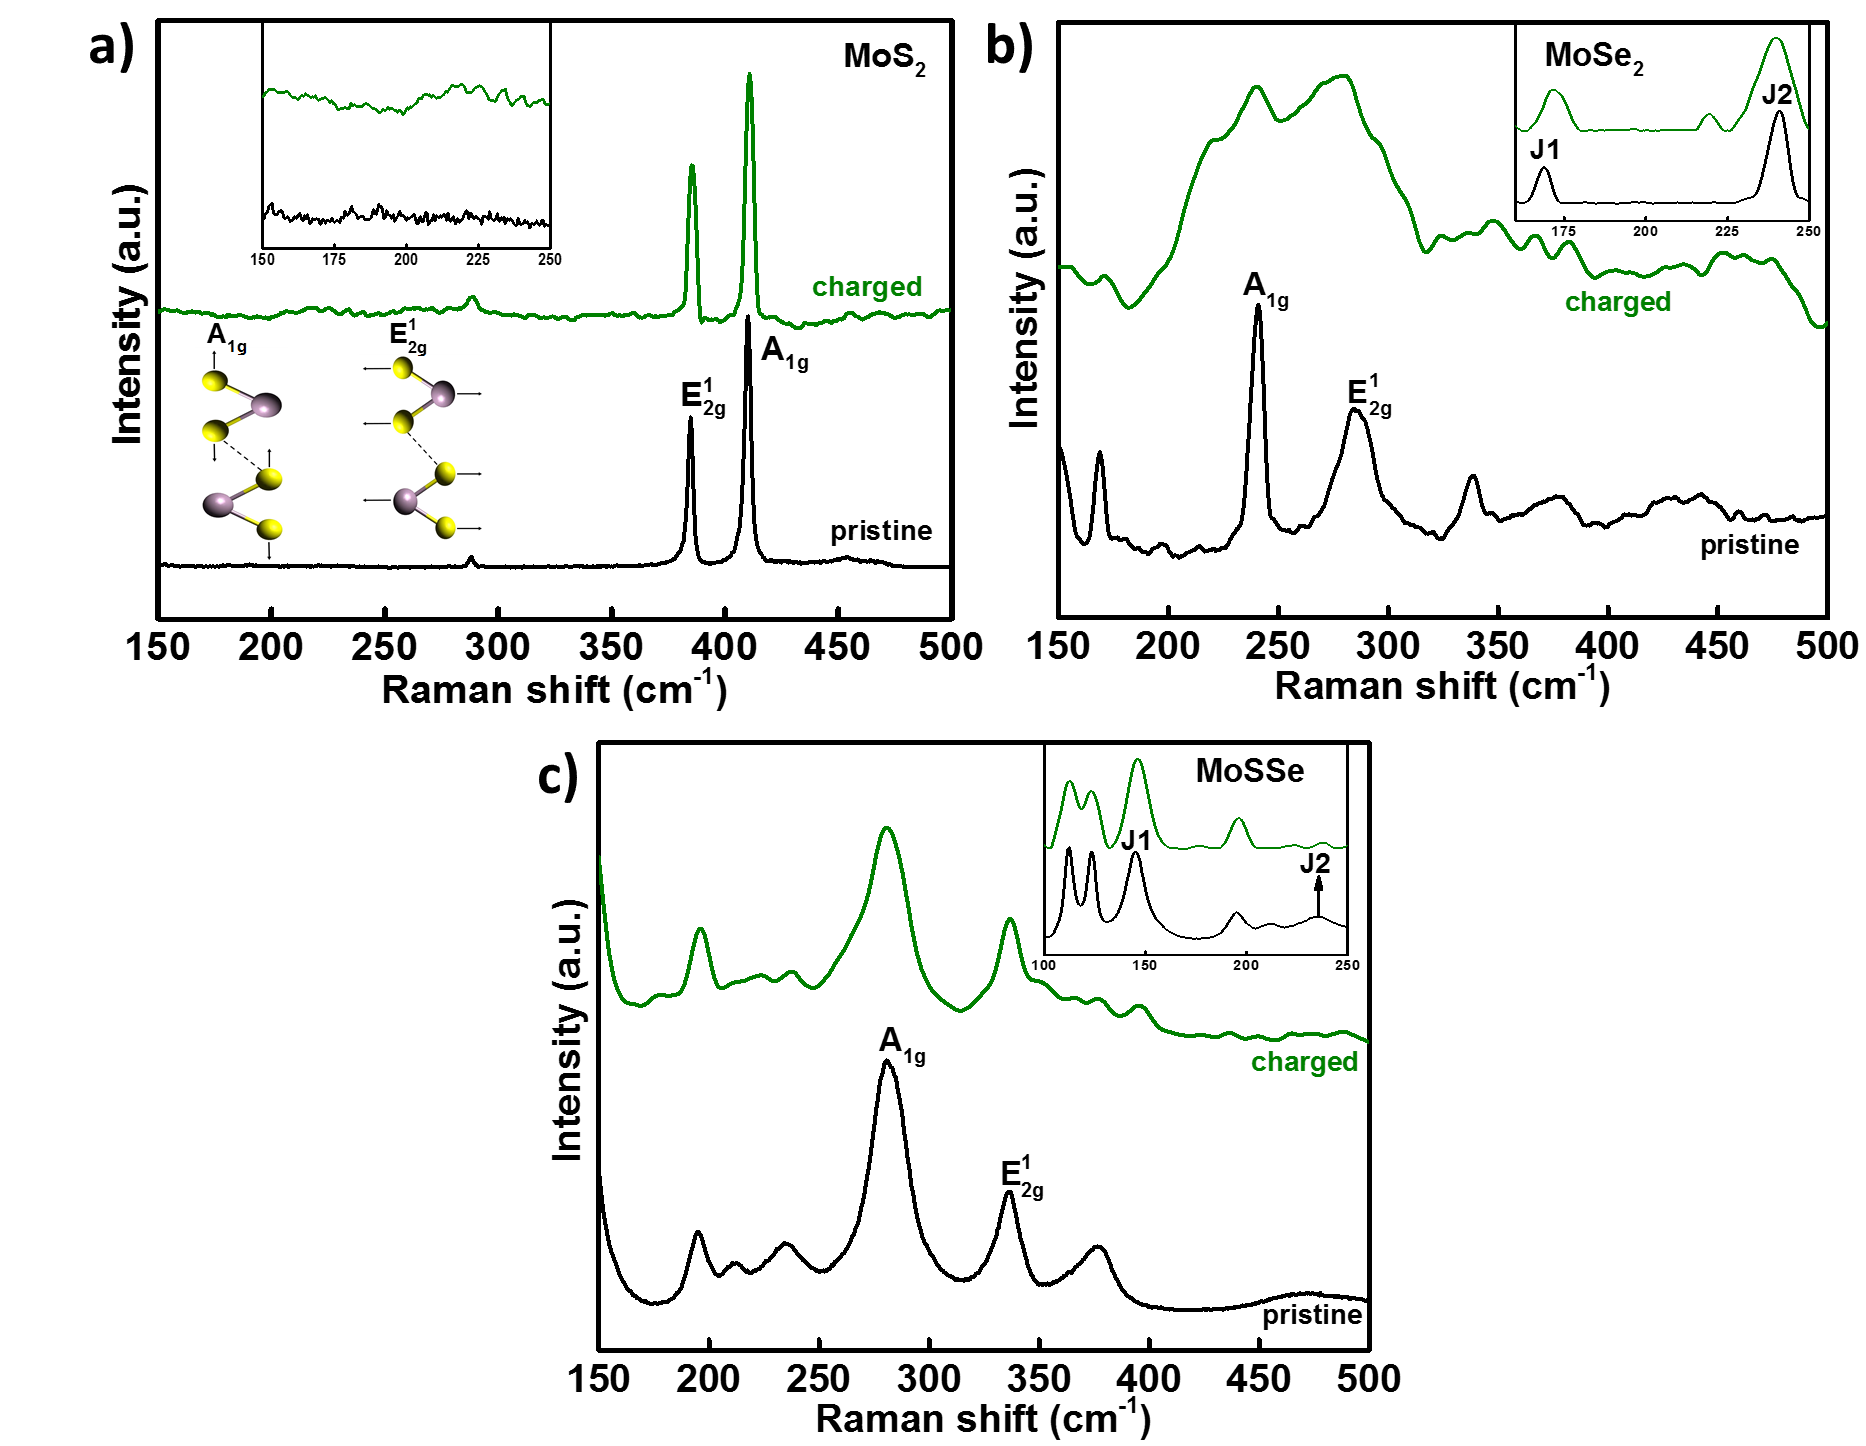
\includegraphics[width=\textwidth]{Figures/chap4fig/fig5}
  \caption{Raman spectra of pristine (black) and charged (green) a)\ce{MoS2}, b) \ce{MoSe2} and c) MoSSe electrodes with position of new Raman active J1 and J2 bands marked along with E$^1_{2g}$ and A$^1_g$ bands.}
  \label{Figures/chap4fig:fig5}
\end{figure}
In addition, the Raman spectra of pristine and charged molybdenum dichalcogenide cathodes were compared to detect shifts in vibrational modes , Figure \ref{Figures/chap4fig:fig5}. Yang and Sharma \textit{et al.} have reported that E$^1_{2g}$ and A$^1_g$ are the most intense vibrational modes for molybdenum dichalcogenides \cite{yang_pressure-induced_2019,sharma_stable_2018}. Peaks corresponding to E$^1_{2g}$ and A$^1_g$ modes for \ce{MoS2} (Figure \ref{Figures/chap4fig:fig5} a) are prominent at 384.6 cm$^{-1}$ and 410.2 cm$^{-1}$ respectively. A$^1_g$ indicates an out-of-plane symmetric displacement of S atoms, whereas E$^1_{2g}$ suggests an in-layer displacement. Also, separation between the two peaks indicates a multi-layer structure, which was clearly observed for all three materials. No significant peak shift or peak broadening was observed for the charged \ce{MoS2} electrode. For 2H \ce{MoSe2} (Figure \ref{Figures/chap4fig:fig5} b), A$^1_g$ is the most intense vibration occurring at a frequency lower than that of E$^1_{2g}$. When the number of layers decreases, the A$^1_g$ mode softens and an increase in the full-width-at-half-maximum (FWHM) is detected. Spectra generated after intercalation/conversion were different from the pristine cathodes because phase conversion from 2H to 1T decreases the molecule's symmetry and more Raman bands get active. The presence of J1 and J2 peaks in addition to E$^1_{2g}$ and A$^1_g$ at lower wavelengths, especially for \ce{MoSe2} and MoSSe (inset, Figure\ \ref{Figures/chap4fig:fig5} b and c), suggest the existence of 1T phase . This agrees with the CV scans and XPS results, where a phase transition was observed for \ce{MoSe2} and MoSSe. Raman results suggest that the symmetry and vibrational modes of \ce{MoSe2}'s crystal lattice changed after repeated charge and discharge cycles. 
\begin{figure}
  \centering
  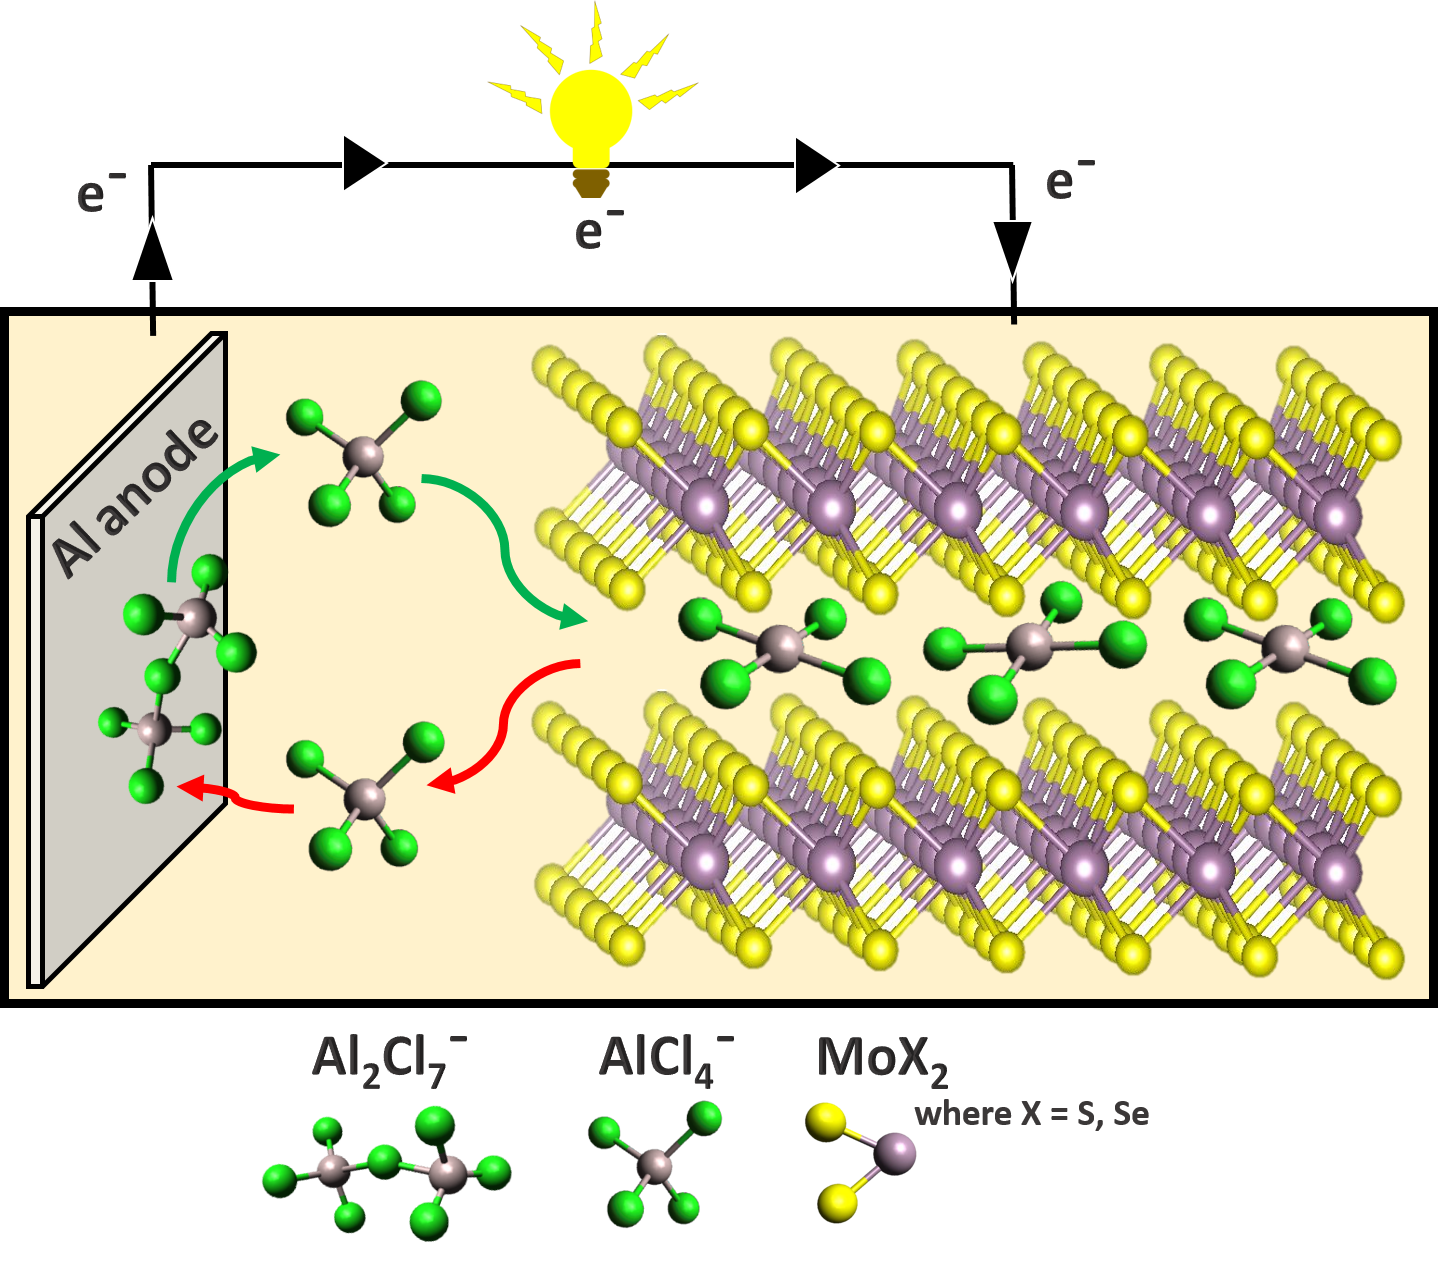
\includegraphics[width=\textwidth]{Figures/chap4fig/graabs}
  \caption{Intercalation of chloroaluminates into the layers of molybdenum dichalcogenides during charge and de-intercalation during discharge.}
  \label{Figures/chap4fig:graabs}
\end{figure}
\section{Summary}
Overall, it was found that despite having similar structures, \ce{MoSe2} achieved higher capacity (stored more energy) than \ce{MoS2} and MoSSe. MoSSe did not have a regular crystalline structure to begin with. The material was unable to store energy reversibly since the cathode structure degraded after a few cycles and the cells became inactive.  

\newpage
\section{Nanostructured molybdenum disulfide and diselenide as cathodes for non-aqueous AIBs} \label{nanmol}
Transition metal dichalcogenides (TMDs) such as \ce{TiS2} and exfoliated \ce{MoS2} flakes have been known as electrochemically active materials since the 1970's due to their fast ionic conductivity \cite{du_superior_2010,whittingham_electrical_1976}. Guodong and his team reported a specific capacity of $\sim$750mAh g$^{-1}$ using re-stacked \ce{MoS2} single layers as a lithium-ion battery anode. The restacking enlarged the c-axis parameter, which denotes its interlayer spacing, and consequently increased the accessible surface area.\\
Nanosized materials increase the contact area between an electrode and the electrolyte. They provide shorter path lengths for both ion diffusion and electron transport in comparison with bulk particles. As a result, the charge/ discharge rate is improved. Since a shorter path length for electronic transport is created, materials having lower electronic conductivity can also be utilised \cite{pitchai_nanostructured_2011}. The high surface area of nanomaterials allows large volume expansion/ contraction associated with ion intercalation/ de-intercalation and prevents cathode pulverisation, which leads to a longer cycle-life \cite{zhang_ultrathin_2015, cong_intrinsic_2015}. Nano-TMDs have been widely explored as electrode materials since they have the potential to improve the electrochemical performance. 
These materials have shown some remarkable performances in LIBs, sodium-ion batteries (SIBs), lithium-sulphur (Li-S) batteries, magnesium-ion batteries (MIBs), etc \cite{xie_mos2/graphene_2015,cao_preparation_2013,dong_insights_2019,li_rechargeable_2018}.\\
Nanostructured \ce{MoS2} has been established as a promising material for energy storage devices. Xie and his group synthesised \ce{MoS2}/ reduced graphene oxide (rGO) nanocomposites as an anode for SIBs \cite{xie_mos2/graphene_2015}. Compared to b-\ce{MoS2} (93 mAh g$^{-1}$), the nanocomposites achieved a high capacity of 702 mAh g$^{-1}$. However, the drawback of these cells was the volume change during charge/discharge cycles. In 2013, Cao \textit{et al.} used \ce{MoS2} coated 3D graphene network (\ce{MoS2}/3DGN) as a binder-free anode material in LIBs \cite{cao_preparation_2013}. The 3DGN improved the electrical contact between the current collector (nickel foam) and the deposited active material, \ce{MoS2}. The cell displayed a discharge capacity of 466 mAh g$^{-1}$ after 10 cycles at a  high current density of 4 A g$^{-1}$. The lithiation process was accompanied by a phase transformation of \ce{Li_xMoS2} from 2H to 1T during first discharge. To determine the significance of the \ce{MoS2} nanoparticles, another composite was prepared using b-\ce{MoS2}. It was observed that due to poor electrical contact between b-\ce{MoS2} and 3DGN, the cell underwent rapid capacity decay. This confirmed that the graphene network provided an efficient pathway for \ce{Li+} exchange. It also showed that the nanostructured \ce{MoS2} had more active edge sites than b-\ce{MoS2}, which resulted in high-performing LIBs. Based on similar principle, Dong \textit{et al.} used \ce{MoS2} nanosheets as an anode material for potassium-ion batteries. They suggested that highly crystalline-\ce{MoS2} displayed higher discharge capacity that poorly-crystallised \ce{MoS2} \cite{dong_insights_2019}. With the rapid progress in research on 2D nanomaterials, large-scale preparation of nanostructured materials at a low cost can be expected for practical applications in the near future. It has been reported that mixing transition metal oxides with nano forms of carbon improves their electrochemical performance in energy storage devices \cite{acerce_metallic_2015-1,zhao_flexible_2015,hu_hierarchical_2015,cao_preparation_2013,ding_facile_2012}. For e.g. Cao \textit{et al.} reported the performance of b-\ce{TiO2} as a cathode in a LIB, which delivered a capacity of 182 mAh g$^{-1}$ and retained 88\% of its specific capacity after 400 cycles \cite{cao_preparation_2013}. The capacity increased to 320 mAh g$^{-1}$ when \ce{TiO2} was mixed with carbon nanotubes (CNT) by Ding and his group \cite{ding_facile_2012}. The cell retained 94\% of its specific capacity after 120 cycles. Table \ref{tmc} compares the performance of bulk transition metals and their nanocomposites in various energy storage devices. 

\begin{sidewaystable}
\centering
\caption{Summary of performances of 2D materials in various energy storage devices.} \label{tmc}
\begin{tabular}{ |p{1.5cm}|p{3.5cm}|p{4.5cm}|p{4.5cm}|p{4.5cm}|}
 \hline 
\textbf{Ref.} & \textbf{Electrode} & \textbf{Electrolyte} & \textbf{Storage capacity} & \textbf{Cycle performance} \\ 
\hline
\cite{acerce_metallic_2015-1} & {Supercapacitors: Metallic 1T \ce{MoS2}} & 0.5M \ce{H2SO4}, \ce{Li2SO4}, \ce{K2SO4} or KCl or EMIm \ce{BF4} & Volumetric capacitance: 400-700 F cm$^{-3}$ & >90\% retained after 5000 cycles\\
\cite{zhao_flexible_2015} & Supercapacitors: MXene/CNTs & 1M \ce{MgSO4} & Volumetric capacitance: 350F cm$^{-1}$ & No degradation after 10000 cycles at 10 A g$^{-1}$\\
\cite{hu_hierarchical_2015} & LIB: \ce{TiO2} & 1M \ce{LiPF6} in a 1: (v:v) mixture of ethylene carbonate and dimethyl carbonate & Specific capacity: 182 mAh g$^{-1}$ at 5C & 87.9\% specific capacity retained after 400 cycles at 5C \\
\cite{cao_preparation_2013} & LIB: \ce{MoS2}/graphene & 1M \ce{LiPF6} in a 1:1 (V:v) mix of ethylene carbonate and dimethyl carbonate & Specific capacity: 466 mAh g$^{-1}$ at 4 A g$^{-1}$ & 566 mAh g$^{-1}$ retained after 50 cycles at 0.5 A g$^{-1}$ \\
\cite{ding_facile_2012} & LIB: \ce{TiO2}/CNT \ce{SnO2}/CNT & 1M \ce{LiPF6} in a 1:1 (w:w) mix of ethylene carbonate and dimethyl carbonate & Specific capacity: 320 mAh g$^{-1}$ for \ce{TiO2}, 580 mAh g$^{-1}$ for \ce{SnO2} at 0.4 A g$^{-1}$ & 93.8\% specific capacity retained after 120 cycles for \ce{TiO2}, 72.4\% retained after 40 cycles at 0.4 A g$^{-1}$ for \ce{SnO2}\\
\cite{xie_mos2/graphene_2015} & SIB: \ce{MoS2}/rGO & 1M \ce{NaClO4} in a 1:1 (V:v) mix of ethylene carbonate and dimethyl carbonate & Specific capacity: 350 mAh g$^{-1}$ at 0.64 A g$^{-1}$ & 227 mAh g$^{-1}$ retained after 300 cycles at 0.32 A g$^{-1}$ \\
\hline
\end{tabular}
\end{sidewaystable}

\subsection{Experimental methods}
The \ce{MoS2} and \ce{MoSe2} nanoflowers were obtained from Tohoku university and used as received. Refer to \ref{slurry},\ref{catprep}, \ref{vac} and \ref{cellass} for slurry and cathode preparation, and cell assembly. 
%Before adding sulfur, pristine \ce{MoO3} (Wako chemicals) was ball-milled for 4 hours. 1 mmol of ascorbic acid (Wako chemicals) as a reducing agent was dissolved in 5 ml of water and the mixture was magnetically stirred for at least 20 minutes under air. Subsequently, 1 mmol of S powder (Sigma-Aldrich) and 0.3 mmol of ball-milled \ce{MoO3} were placed in the reactor. Lastly, 5 ml of ascorbic acid aqueous solution was injected into the reactor vessels containing the powder mixture. The sealed reactor was kept at 400$^{\circ}$C in a tube furnace for 30 minutes. After heating, the samples were collected in the same procedure as above.

\subsection{Results and discussion}
In this chapter \ce{MoS2} and \ce{MoSe2} nanoflowers were used as cathodes in non-aqueous AIBs. The \ce{MoS2} and \ce{MoSe2} cells displayed a capacity of $\sim$60 and $\sim$100 mAh g$^{-1}$ at a current rate of 50 mAh g$^{-1}$ after 5 and 10 cycles respectively. The performance was significantly better that previously reported by Li and his group \cite{li_rechargeable_2018}. Figures \ref{Figures/chap4fig:nanocdccecv} a-b and \ref{Figures/chap4fig:nanocdccecv} c-d show the charge/ discharge curves and CEs of \ce{MoSe2} and \ce{MoS2} cells respectively. It was observed that the discharge curves for both \ce{MoSe2} and \ce{MoS2} looked similar to their bulk counterparts, shown in Figure \ref{Figures/chap4fig:mox2bulkcdccv} a and b. Nano \ce{MoSe2} (n-\ce{MoSe2}) displayed discharge voltage plateaus at 1.9 V. There was also a visible voltage bend during discharge at 0.75 V. A plateau was observed during charge at 2.0 V (similar to b-\ce{MoSe2} seen in Figure \ref{Figures/chap4fig:mox2bulkcdccv} b). In Figure \ref{Figures/chap4fig:nanocdccecv} the CV curves for \ce{MoSe2} displayed redox peaks at potentials corresponding to the voltage plateaus in the charge and discharge curves confirming the presence of redox couples and possibility of ion intercalation or conversion. The discharge capacity of n-\ce{MoSe2} decreased from 90 to 60 mAh g$^{-1}$ after 10 cycles. It seemed the nanostructured \ce{MoSe2} was unable to store charge reversibly unlike its bulk counterpart. Interestingly, the CE of both materials was low at $\sim$40-50\%. This meant that the total charge extracted from the cells was lower than the charge put into them over a full cycle i.e. not all ions that were inserted into the layers were extracted out. Low CE may also indicate the presence of side reactions due to presence of impurities in the electrode and the electrolyte. The behaviour of n-\ce{MoS2} was similar to b-\ce{MoS2}. Voltage bends at 2.1 and 0.65 V were observed during discharge (compare Figure \ref{Figures/chap4fig:nanocdccecv} a and Figure \ref{Figures/chap4fig:mox2bulkcdccv} a). However, the voltammogram did not display any redox peaks, unlike bulk-\ce{MoS2} (O1, O2, R1, R2 and R3 in Figure \ref{Figures/chap4fig:mox2bulkcdccv} c). The CV scans of \ce{MoS2} and \ce{MoSe2} displayed interesting results which have been listed below.  
\begin{itemize}
\item CV of n-\ce{MoS2} had a larger area than b-\ce{MoS2}. Furthermore, the redox peaks which were clearly visible in the bulk were absent in the n-\ce{MoS2}. This suggested that charge storage in n-\ce{MoS2} was non-Faradaic in nature unlike b-\ce{MoS2}. 
\item CV of \ce{MoSe2} revealed the presence of redox processes. There were significant oxidation and reduction peaks at 2.1 V (O'2 in bulk) 1.6 (R'2 in bulk) and 1.7 V (R'1 in bulk) respectively. These peaks corresponded well with the b-\ce{MoSe2}. However, the peak at 1.8 V (O'1) was missing in the n-\ce{MoSe2}. 
\end{itemize}
Also, there was a significant difference between the charging and the discharging curves (same as bulk) , which was attributed to the electrochemical polarization taking place at the cathode.
\begin{figure}[h!]
  \centering
  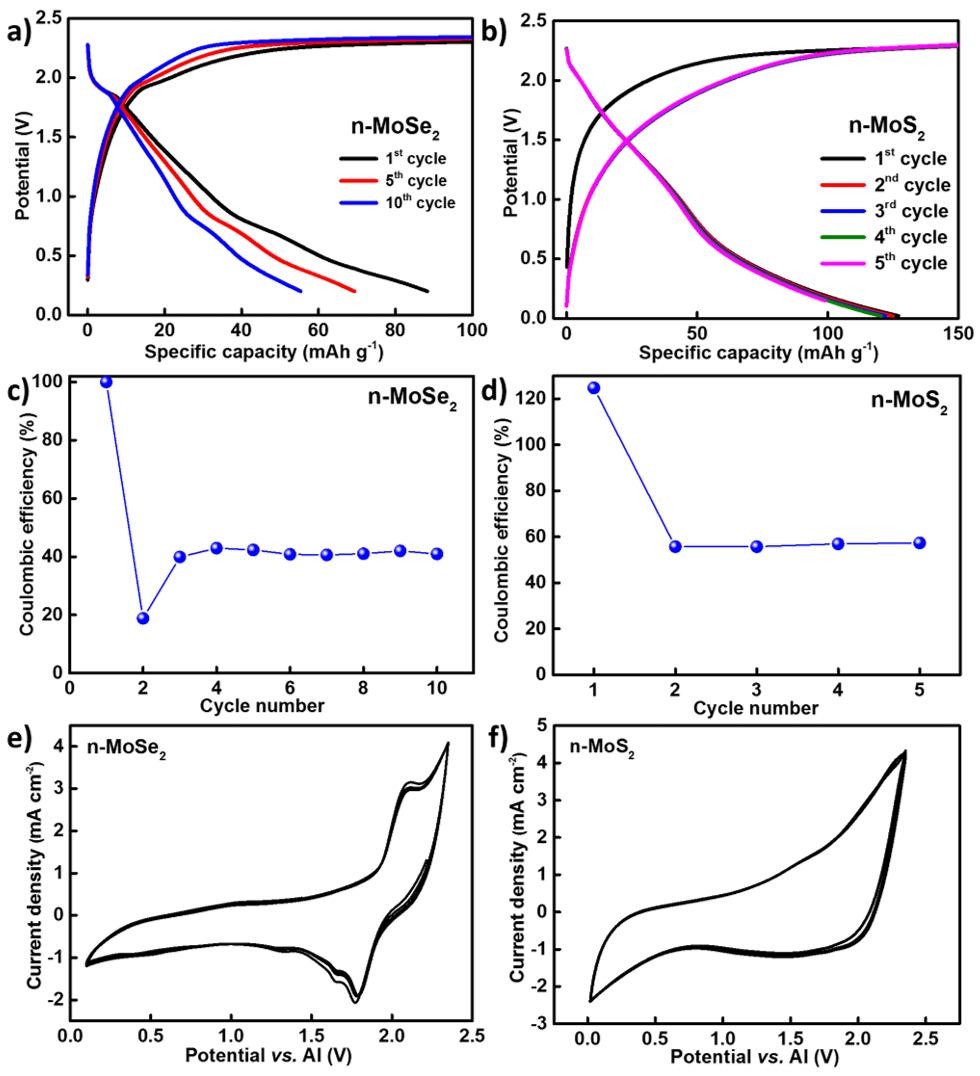
\includegraphics[width=\textwidth]{Figures/chap4fig/nanocdccecv}
    \caption{Galvanostatic charge and discharge curves of a) Al/n-\ce{MoSe2} and b) Al/n-\ce{MoS2} cell. CE for c) n-\ce{MoSe2} and d) n-\ce{MoS2} cell. Cyclic voltammogram of e) n-\ce{MoSe2} and f) n-\ce{MoS2} within the electrochemical window of 0.02 and 2.35 V.}
  \label{Figures/chap4fig:nanocdccecv}
\end{figure}

\begin{figure}[th!]
\centering
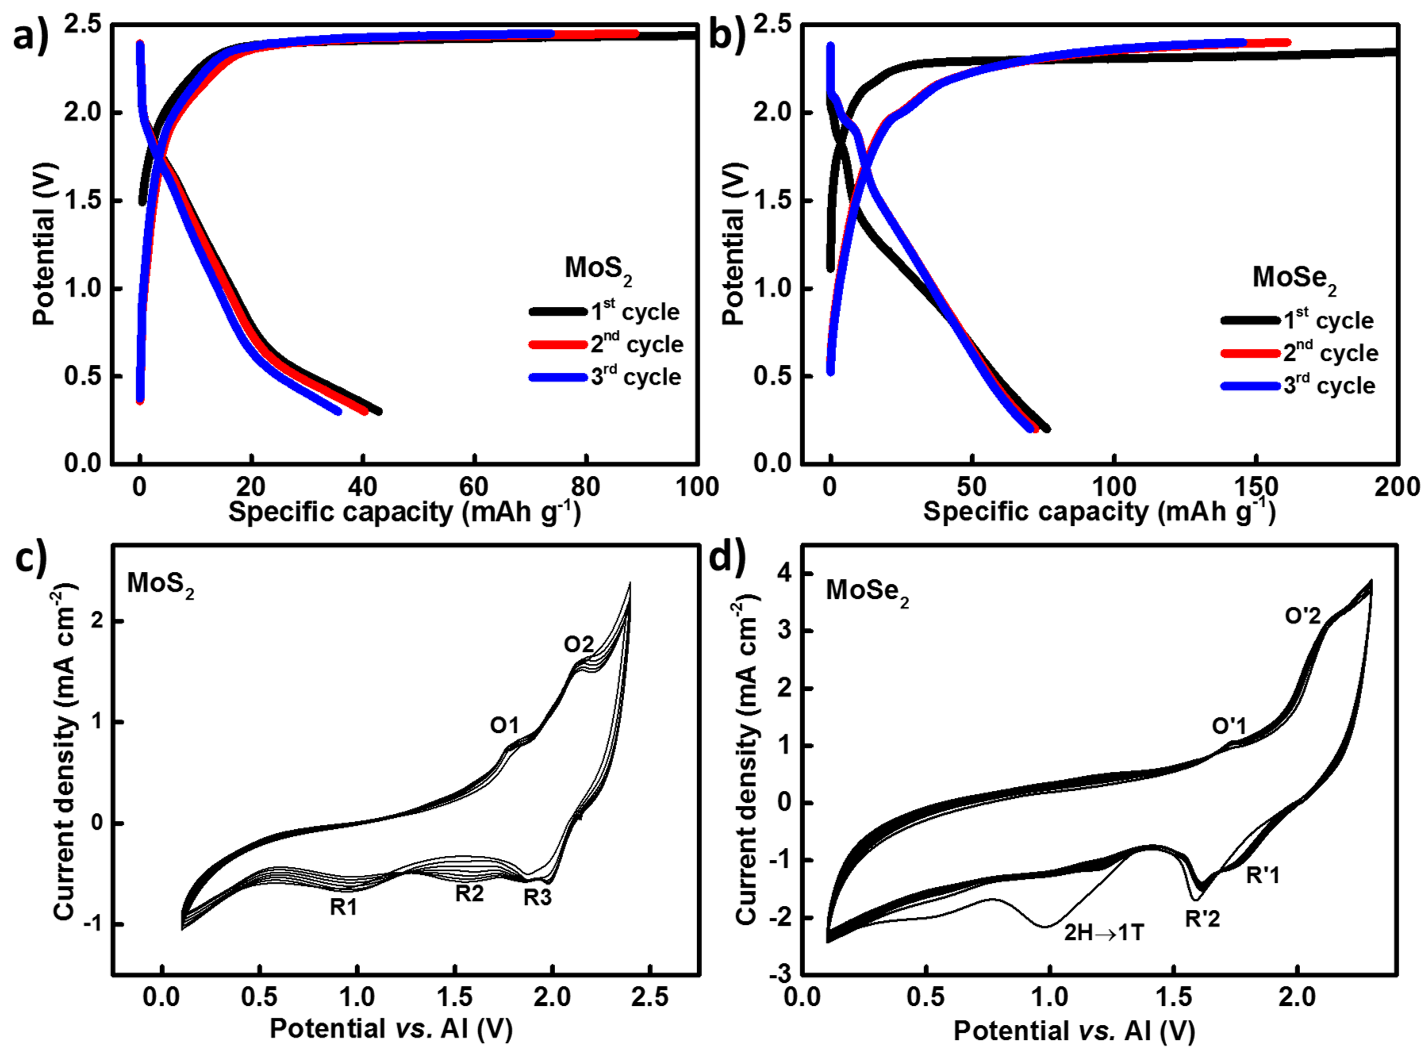
\includegraphics[width=\textwidth]{Figures/chap4fig/mox2bulkcdccv}
\caption{Galvanostatic charge and discharge curves of a) bulk Al/\ce{MoS2} and b) bulk \ce{MoSe2} cell at a current rate of 50 mA g$^{-1}$. CV scans of bulk c) \ce{MoS2} and d) \ce{MoSe2} with distinct redox peaks marked .}
\label{Figures/chap4fig:mox2bulkcdccv}
\end{figure}

\begin{figure}[h!]
  \centering
  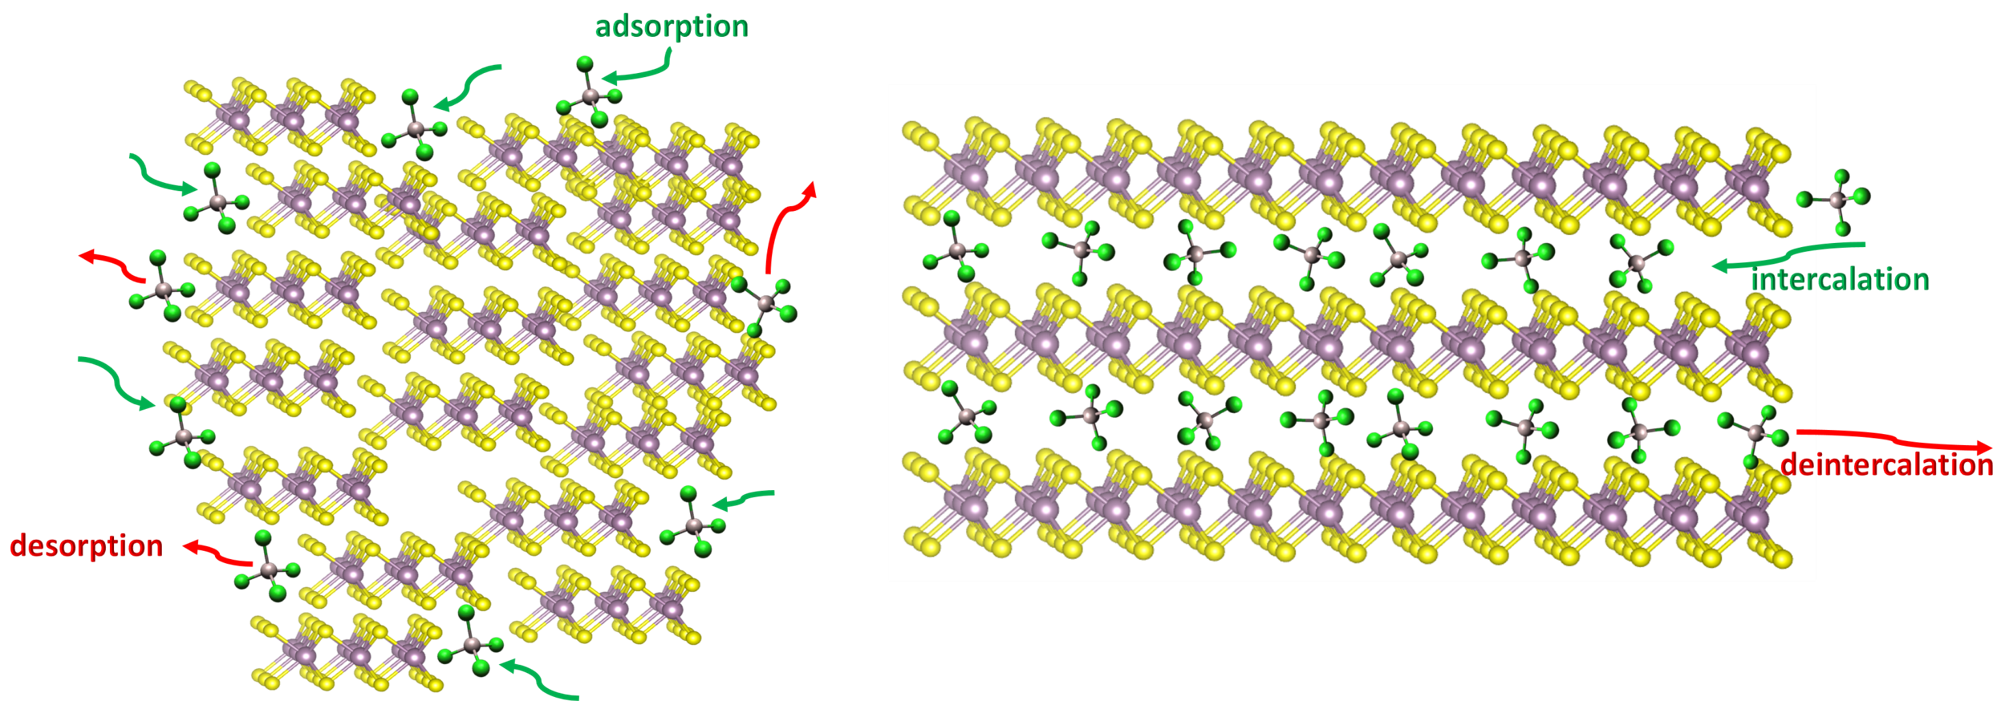
\includegraphics[width=\textwidth]{Figures/chap4fig/bulknano}
    \caption{Schematic illustration of charge storage by \ce{MoX2} nanoflowers (left) and bulk material (right).}
  \label{Figures/chap4fig:bulknano}
\end{figure}

\subsection{Summary}
Overall, it was found that the bulk molybdenum dichalcogenides performed better than the nanostructured materials. Despite having a larger surface area, it seems that the nanostructured dichalcogenides did not have enough layers to reversibly accommodate the \ce{AlCl4-} ions during charge. Agglomeration of the nanoparticles might have resulted in the poor performance of the nanoflowers. 
The nanomaterials used in this chapter might behave differently if:
\begin{itemize}
\item New nanocomposites are made using carbon-based materials (reduced graphene oxide, CNTs), which would not only improve the contact between the current collector and the active material, but also enhance the cell's capacity by phase transformation, which wasn't observed in the nanoflowers
\item Increasing the number of layers present in the molybdenum dichalcogenides i.e. the nanoflowers tested above have very few layers, which might have resulted in faster agglomeration of the active material resulting low cell efficiencies and low discharge capacities. The number of layers can be increased by modifying the synthesis procedure. It will be interesting to study the performance of the nanoflowers with more layers.
\end{itemize}
